\chapter{Theoretical Background}
\label{cha:theory}

\section{Statistical thermodynamics and Free Energy}
\label{sec:freeE}

The formulation of the problem of free energy estimation starts with the Hamiltonian
\begin{equation}
  \textbf{H}(\textbf{x},\textbf{p})=\sum_{i=0}^{N}\frac{p_{i}^{ 2}}{2 m_i} + U(\textbf{x})
  \label{eq:lagrangian}
\end{equation}
of an arbitrary chemical system, where $(\textbf{x},\textbf{p})$ denotes a point in the phase space of the N-particle system of interest with atomic coordinates $\textbf{x}=(x_1, ..., x_N)$, momenta $\textbf{p}=(p_1,...,p_N)$ and masses $(m_1,...,m_N)$. $U(\textbf{x})$ is the potential energy given by any quantum chemical method or force field. If the canonical (N,V,T)-ensemble of such a system is sampled, for example by means of Langevin dynamics or Monte Carlo simulations, the probability distribution $\rho(\textbf{x})$ in the configuration space $\textbf{x}$ follows the Boltzmann distribution
\begin{equation}
  \rho(\textbf{x})=\frac{e^{-\beta U(\textbf{x})}}{\int e^{-\beta U(\textbf{x})} d\textbf{x}}=Z^{-1}e^{-\beta U(\textbf{x})}
  \label{eq:boltzmann}
\end{equation}
were $Z$ denotes the \textit{canonical partition function} and $\beta=(k_B T)^{-1}$ the inverse temperature with Boltzmann constant $k_B$.\autocite{chipot2007free}
%By acting as normalization constant to ensure $\int\rho(x)dx=1$, the partition function is the central quantity of statistical thermodynamics, relating macroscopic thermodynamic quantities to the microscopic details of a system.
In this thesis we will focus on alchemical transformations, $A\longrightarrow B$, which are represented by a small set of collective variables (CV's)
\begin{equation}
 \xi_1(\textbf{x}) : \mathbb{R} ^{3N} \to \mathbb{R}, ..., \xi_n(\textbf{x}) : \mathbb{R} ^{3N} \to \mathbb{R}
\end{equation}
that are sufficient to distinguish between key states of interest.
In this framework the probability distribution can be expressed by
\begin{equation}
  \rho(\xi)=\int \delta[\xi'(\textbf{x})-\xi]\rho(\textbf{x})d\textbf{x}=\braket{\delta [\xi'(\textbf{x})-\xi]}_\xi
  \label{eq:rho}
\end{equation}
where $\braket{}_\xi$ denotes the $\xi$-conditioned marginal distribution. The Helmholtz free energy $A$, i.e. potential of the canonical ensemble, is defined as
\begin{equation}
  A(\xi) = -\beta^{-1}\ln \rho(\xi)
  \label{eq:free energy}
\end{equation}
Note that the shape of the obtained free energy surface (FES) is not gauge invariant against the choice of CV function $\xi$. This is, however, no concern in the calculation of free energy differences, because the CV dependent feature is integrated out to obtain the probability that the system occupies state A or B.\autocite{bal2020free}
\begin{equation}
  \Delta A_{A\rightarrow B} = -\beta^{-1}\ln \frac{\int_B \rho(\xi)d\xi}{\int_A \rho(\xi)d\xi}=-\beta^{-1}\ln \frac{p_B}{p_A}
  \label{eq:free energy diff}
\end{equation}
However, in computer simulations the direct phase-space integrals used in equation \ref{eq:boltzmann} and \ref{eq:rho} are impossible to calculate.\autocite{chipot2007free} Instead the time average $P(\xi)$ is computed by monitoring $\xi$ during the simulation.
\begin{equation}
  P(\xi)=\lim_{t\rightarrow \infty}\frac{1}{t} \int_0^t \rho[\xi (t')] dt'
  \label{eq:ergodic}
\end{equation}
In practice, $P(\xi)$ is approximated as a histogram along the reaction coordinate with bins of fixed size.
Assuming that the system at hand behaves \textit{ergodic}, i.e. every point in phase space is visited during a infinitely long simulation, the ensemble average $\rho(\xi)$ converges to the time average $P(\xi)$ of one system.
However, transitions of high energy barriers during chemical reactions are typically rare events, that might happen on timescales far beyond what is feasible to compute, especially on accurate quantum chemical level of theory. Therefore most processes, for example in biochemical context, behave \textit{quasinonergodic}.
The problem of calculating accurate free energy differences hence really consists in adequate sampling of regions with high free energy (transition states) along the reaction coordinate.

For this purpose several \textit{enhanced sampling} algorithms were proposed.\autocite{jiang2010free, sugita1999replica,den2000thermodynamic, kastner2011umbrella, ciccotti2005blue, barducci2008well}
In this work we will focus on CV-based approaches, that alter the potential energy $U(\textbf{x})$ of the system in a way, that increases the time spent in important regions of configuration space during a simulation. One of the oldest and simplest methods to achieve the same is \textit{Umbrella Sampling} (US)\autocite{kastner2011umbrella}, which will be introduced in the following section.
The main focus of this work lies on \textit{Adaptive Biasing Methods} \autocite{barducci2011metadynamics,comer2015adaptive, lesage2017smoothed}, which aim for uniform sampling along the reaction coordinate by an history dependent biasing term (section \ref{sec:adaptive biasing}).
\newpage

\section{Umbrella Sampling (US)}
In its most common form US introduces a fixed harmonic bias potential of the form
\begin{equation}
  U_i^B(\xi) = \frac{k_i}{2}(\xi(t)-\xi_i)^2 \label{eq:US bias}
\end{equation}
where the index i indicates a given bias window along the reaction coordinate with force constant $k_i$.\autocite{kastner2011umbrella} From simulations in window i the biased probability distribution $P_i^B(\xi)$ is obtained
\begin{equation}
\begin{split}
  P_i^B(\xi) &= \frac{\int d\textbf{x} e^{-\beta (U(\textbf{x})+U_i^B(\xi(\textbf{x})))}\delta[\xi'(\textbf{x})-\xi]}
  {\int d\textbf{x} e^{-\beta (U(\textbf{x})+U_i^B(\xi(\textbf{x})))}} \\
             &= \frac{e^{-\beta U_i^B(\xi(\textbf{x}))}}{\int e^{-\beta (U(\textbf{x})+U_i^B(\xi(\textbf{x})))}d\textbf{x}} \int d\textbf{x} e^{-\beta U(\textbf{x})}\delta[\xi'(\textbf{x})-\xi]
\end{split}
\end{equation}
where $Z_B$ denotes the partition function of the biased potential energy $U(\textbf{x})+U_i^B(\xi(\textbf{x}))$.
Using equation \ref{eq:boltzmann} and \ref{eq:rho} the connection of $P_i^B$ to the unbiased probability distribution $P_i^0$ can be derived.
\begin{equation}
\begin{split}
  P_i^0(\xi) &= P_i^B(\xi)e^{\beta U_i^B(\xi)}\frac{\int e^{-\beta (U(\textbf{x})+U_i^B(\xi(\textbf{x})))}d\textbf{x}} {\int e^{-\beta U(\textbf{x})}d\textbf{x}} \\
  &= P_i^B(\xi)e^{\beta U_i^B(\xi)}\frac{Z_B}{Z_0}
\end{split}
\end{equation}
Inserting into equation \ref{eq:free energy} gives the unbiased free energy
\begin{equation}
  \begin{split}
  A_i(\xi) &= -\beta^{-1}\ln P_i^B(\xi) - U_i^B(\xi) - \beta^{-1}\ln\frac{Z_B}{Z_0} \\
           &= A_B(\xi) - U_i^B(\xi) - F_i \label{eq:A US}
  \end{split}
\end{equation}
The last therm of equation (\ref{eq:A US}) is the free energy difference between the unbiased and biased system. Since it is a constant it can be ignored in the calculation of free energy differences from a single window.

However, in order to enhance sampling along the reaction coordinate usually a stratification strategy is applied simulating multiple overlapping windows. In this case the global unbiased distribution of all combined windows is calculated with the \textit{Weighted Histogram Analysis Method} (WHAM).\autocite{kumar1992weighted} The goal of WHAM is to choose the weights $p_i(\xi)$ in order to minimize the statistical error of the global probability distribution of S combined windows
\begin{equation}
  P^U(\xi)=\sum_i^{S} p_i(\xi)P_i^0(\xi)
\end{equation}
under the constraint $\sum p_i = 1$. This is achieved by the iterative solution of the self-consistent WHAM equations
\begin{equation}
  p_i(\xi) = \frac{N_i \e^{-\beta_i U_i^B(\xi)+\beta_i F_i}}{\sum_j^S N_j \e^{-\beta_j U_j^B(\xi)+\beta_j F_j}} \label{eq:WHAM 1}
\end{equation}
\begin{equation}
  \e^{-\beta_i F_i} = \int P^U(\xi)\e^{-\beta_i U_i^B (\xi)}d\xi
  \label{eq:WHAM 2}
\end{equation}
where $F_i$ enters equation (\ref{eq:WHAM 1}) and $P^U$ enters equation (\ref{eq:WHAM 2}). $N_i$ is the number of samples collected in window i.
The biggest advantage of this approach is that all windows can be simulated in parallel on different computing nodes and only have to be combined once to solve the WHAM equations. This way extensive sampling of the reaction coordinate can be obtained efficiently.
However, the biasing potentials have to be chosen manually for each window, requiring some knowledge of the free energy surfaces at hand prior to the simulation.
Additionally, up to 50\% of the simulation time can be spent in overlapping regions of ascending windows.\autocite{comer2015adaptive}
In the next section we will look at different approaches, that eliminate both drawbacks by replacing equation \ref{eq:US bias} with an time dependent term, which evolves during the simulation to achieve uniform sampling of the reaction coordinate.

\newpage
\section{Adaptive Biasing Methods}
\label{sec:adaptive biasing}

Instead of dividing the reaction coordinate in several windows, with adaptive biasing methods the free energy can be estimated from one single simulation. For this purpose the systems dynamics are biased towards states corresponding to large values of the free energy along the transition coordinate via a history-dependent biasing potential. In contrast to other importance sampling strategies like umbrella sampling, this methods require less knowledge of the free energy surface at hand prior to the simulation, because the bias is not chosen manually. Instead, the biasing potential automatically adapts during the simulation to enable diffusive behavior along the transition coordinate.\autocite{comer2015adaptive, barducci2011metadynamics}

There are multiple adaptive biasing methods available, only differing in the construction of the bias. Potential based methods like metadynamics (MtD) disfavor already visited states by accumulating repulsive potentials along the CV (section \ref{sec:metaD}), while adaptive biasing force (ABF) methods compensate the mean force along the reaction coordinate to obtain uniform sampling (section \ref{sec:ABF}). Finally, as discussed in section \ref{sec:eABF}, using an extended Lagrangian, the technical requirements of ABF can be lifted without loosing its rigorous convergence behavior.\autocite{lesage2017smoothed} Additionally, this framework enables the combination of repulsive Mtd-potentials with ABF (meta-eABF/WTM-eABF), to unite the benefits of both approaches.\autocite{fu2018zooming,fu2019taming}

Although not necessary, stratification can increase the convergence of all adaptive biasing methods significantly. However, in contrast to US simulations, no WHAM and hence no overlap between ascending windows is required. For example in ABF simulations the global PMF can be recovered by simply joining the force estimates of all simulations.\autocite{comer2015adaptive} Multiple-Walker strategies can also be trivially implemented, by letting more than one simulation contribute to the same biasing potential, as will be discussed in section \ref{sec:MW}.\autocite{minoukadeh2010potential}

In principle adaptive biasing methods only rely on sampling of the canonical ensemble, which will be obtained using Langevin dynamics in this work. However, all methods can also be applied in combination with other MD or MC engines. A schematic procedure of adaptively biased Langevin dynamics is given in Algorithm \ref{alg:ABM}.

\begin{algorithm}[H]
  \caption{Velocity Verlet integrator for adaptively biased Langevin dynamics with atomic masses $\textbf{M}$, coordinates $\textbf{x}(t)$, momenta $\textbf{p}(t)$, potential $U(\textbf{x}(t))$, forces $F(\textbf{x}(t))$ and friction coefficient $\gamma$,}
  \label{alg:ABM}
    \begin{algorithmic}
      \WHILE{$t < t_{end}$}
        \STATE
        \STATE $\textbf{p}(t+\frac{1}{2}\Delta t) \leftarrow \textbf{p}(t) + \frac{1}{2} \bigl(F(\textbf{x}(t))dt-\gamma \textbf{M}^{-1}\textbf{p}(t) dt + \sqrt{2\gamma\beta^{-1}}dW_t \bigr)$
        \STATE $\textbf{x}(t+\Delta t) \leftarrow \textbf{x}(t) + \frac{2}{2+\gamma dt}\textbf{M}^{-1} \textbf{p}(t+\frac{1}{2}\Delta t) dt$
        \STATE /* Langevin dynamics
        \STATE
        \STATE $F(\textbf{x}(t+\Delta t)) \leftarrow -\nabla U(\textbf{x}(t+\Delta t))$
        \STATE /* get physical QM/MM forces
        \STATE
        \STATE $\xi \leftarrow f(\textbf{x}(t+\Delta t))$
        \STATE /* Calculate reaction coordinate from Cartesian coordinates
        \STATE
        \IF{$\xi_{min}\leq\xi\leq\xi_{max}$}
          \STATE
          \STATE $F_{B}(\xi, t+\Delta t))\leftarrow F_{B}(\xi, t))+\Delta F_{B}(\xi,t+\Delta t))$
          \STATE /* update history dependent bias force along reaction coordinate incrementally
          \STATE
          \STATE $F(\textbf{x}(t+\Delta t)) \leftarrow -\nabla U(\textbf{x}(t+\Delta t)) + F_{B}(\xi, t+\Delta t))\nabla\xi$
          \STATE /* Add biasing force to physical force
          \STATE
        \ELSE
          \STATE
          \STATE $F(\textbf{x}(t+\Delta t)) \leftarrow F(\textbf{x}(t+\Delta t)) + k\min(|\xi-\xi_{min}|,|\xi-\xi_{max}|)\nabla\xi$
          \STATE /* confine system to range of interest with harmonic constraining force
          \STATE
        \ENDIF
        \STATE
        \STATE $\textbf{p}(t+\Delta t) = \frac{2 - \gamma dt}{2+\gamma dt} \textbf{p}(t+\frac{1}{2}\Delta t) - \frac{1}{2} \bigl(F(\textbf{x}(t+\Delta t))dt-\gamma \textbf{M}^{-1}\textbf{p}(t+\frac{1}{2}\Delta t)) dt + \sqrt{2\gamma\beta^{-1}}dW\bigr)$
        \STATE /* Langevin dynamics
        \STATE
      \ENDWHILE
      \STATE /* get unbiased free energy
    \end{algorithmic}
\end{algorithm}

\newpage
\subsection{(Well-Tempered) Metadynamics (MtD/WTM)}
\label{sec:metaD}

MetaD biases a systems dynamic towards undersampled regions along the reaction coordinate $\xi(\textbf{x})$, by accumulating repulsive potentials in regions that have already been visited.\autocite{barducci2011metadynamics} The bias potential is typically build by a superposition of repulsive Gaussian kernels and can be written
\begin{equation}
  U_{MtD}(\xi,t)= \sum_{k<\frac{t}{\tau_G}} \tau_G \omega \exp\biggr(-\sum_{i=1}^{N_{dim}} \frac{1}{2\sigma_{i}^{2}} (\xi_{i}(\textbf{x})-\xi_{i}(\textbf{x},t_k))^2 \biggl),
  \label{eq:U_mtD}
\end{equation}
with deposition rate $\tau_G$, Gaussian height $\omega=W/\tau_G$ and variance $\sigma^2$ as free input parameters. Over the course of a simulation the bias potential fills local minima along the reaction coordinate until the systems evolution finally resembles a Brownian motion along the flattened free energy surface. The converged bias potential provides an unbiased estimate of the underlying free energy surface
\begin{equation}
  A(\xi) = -U_{MtD}(\xi, t \to \infty) + C
\end{equation}
To avoid oscillation of $U_{MtD}$ around the correct free energy, Well-Tempered metadynamics (WTM)\autocite{barducci2008well} introduces an additional scaling factor of the Gaussian height
\begin{equation}
  \omega(\xi,t) = \frac{W}{\tau_G}\exp\biggl(-\frac{U_{WTM}(\xi,t)}{k_B \Delta T} \biggr)
  \label{eq:WTM}
\end{equation}
to ensure an decrease of $\omega$ over time and smooth convergence of the Well-Tempered bias potential $U_{WTM}(\xi,t)$. The WTM potential does not fully compensate the free energy barrier, but can be controlled by parameter $\Delta T$. For $\Delta T \to 0$ the bias is zero and ordinary MD is recovered, whereas the limit $\Delta T \to \infty$ corresponds to normal MtD. Figure~\ref{fig:metaD} shows a numerical example of the effect of $U_{MtD}$ and $U_{WTM}$ on the effective free energy energy surface that is sampled over the course of a simulation.

To again obtain the unbiased PMF from $U_{WTM}(\xi,t)$ it has to be scaled with an according correction factor to compensate the effect of $\Delta T$:
\begin{equation}
A(\xi) = -\frac{T+\Delta T}{\Delta T}U_{WTM}(\xi, t)
\end{equation}
Despite its appealing theoretical and practical simplicity MtD and WTM both suffer from a rather big set of free parameters ($W$, $\tau_G$, $\sigma$ and $\Delta T$). All of them have significant impact on the outcome of the simulation and have to be chosen carefully. If the bias potential builds up too fast the system is driven far away from equilibrium and the obtained free energy estimate is wrong. Small parameters on the other hand result in bad convergence behavior and inefficient sampling.\autocite{laio2005assessing}
The next section will look into ABF, which is less dependent on free parameters and stands on a more rigorous mathematical framework.

\begin{figure}[H]
    \centering
    \subfloat[Metadynamics]{{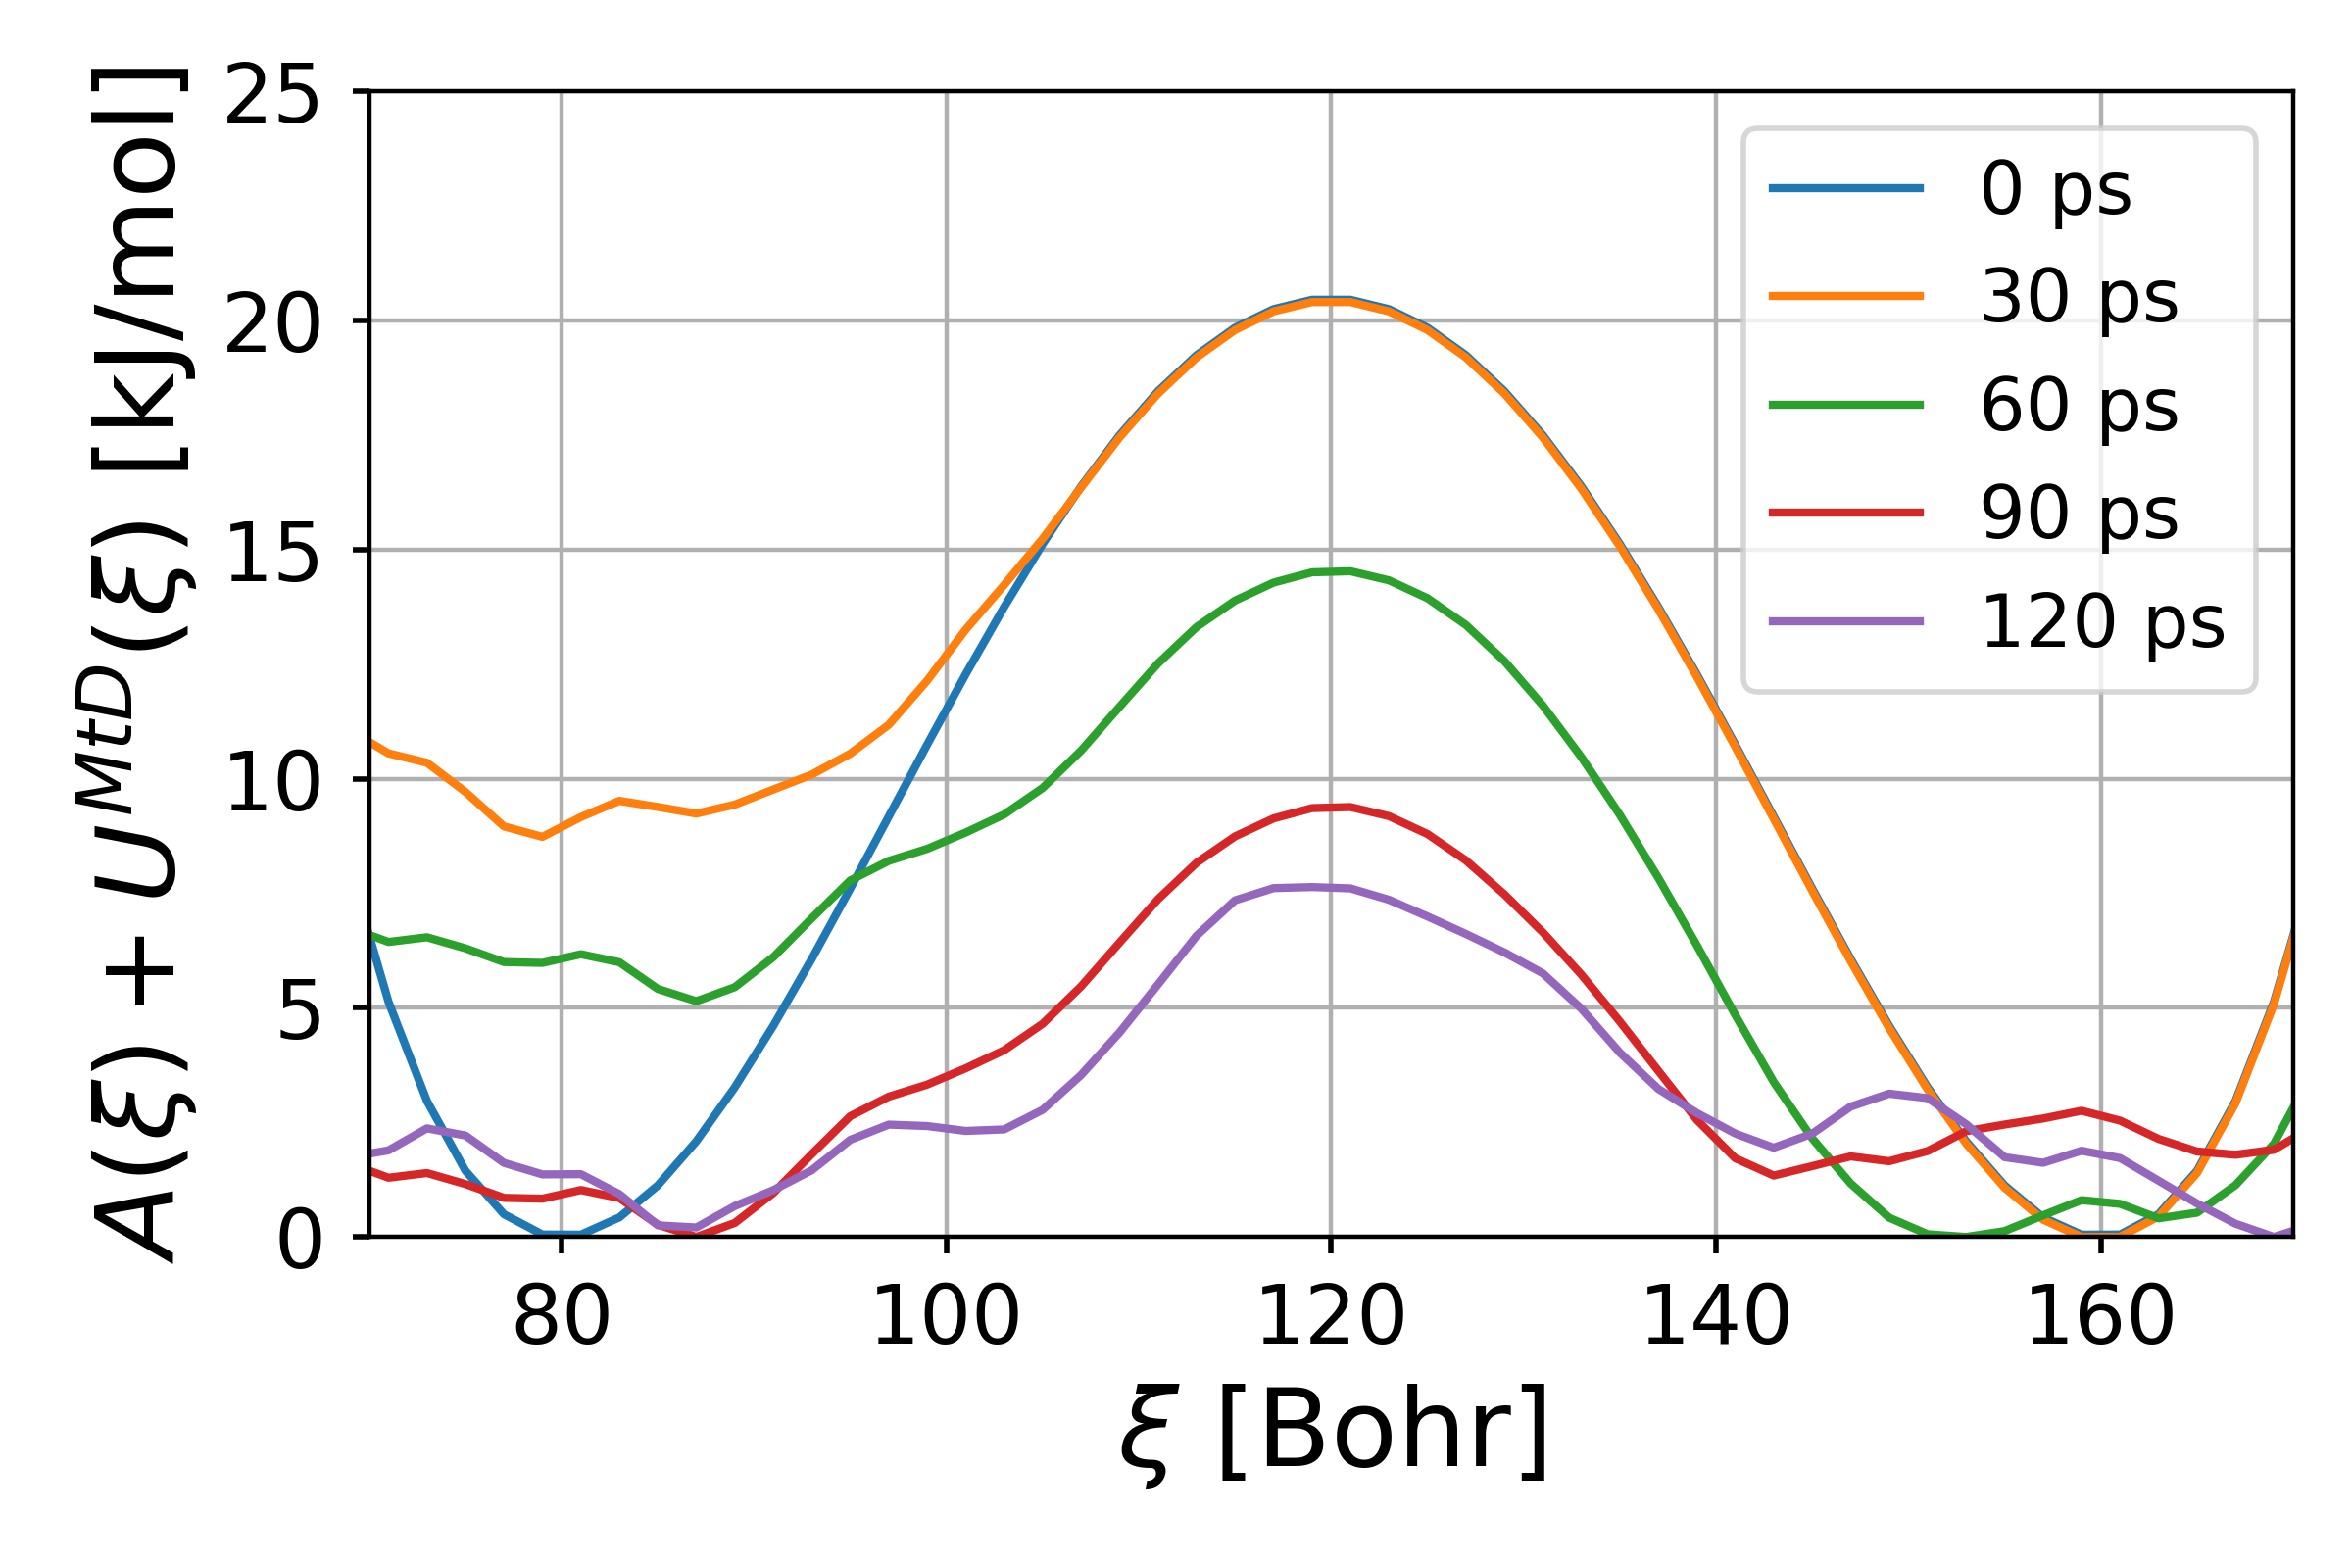
\includegraphics[width=0.49\textwidth]{bilder/metaD_eff_pot} }}
    \subfloat[Well-Tempered Metadynamics]{{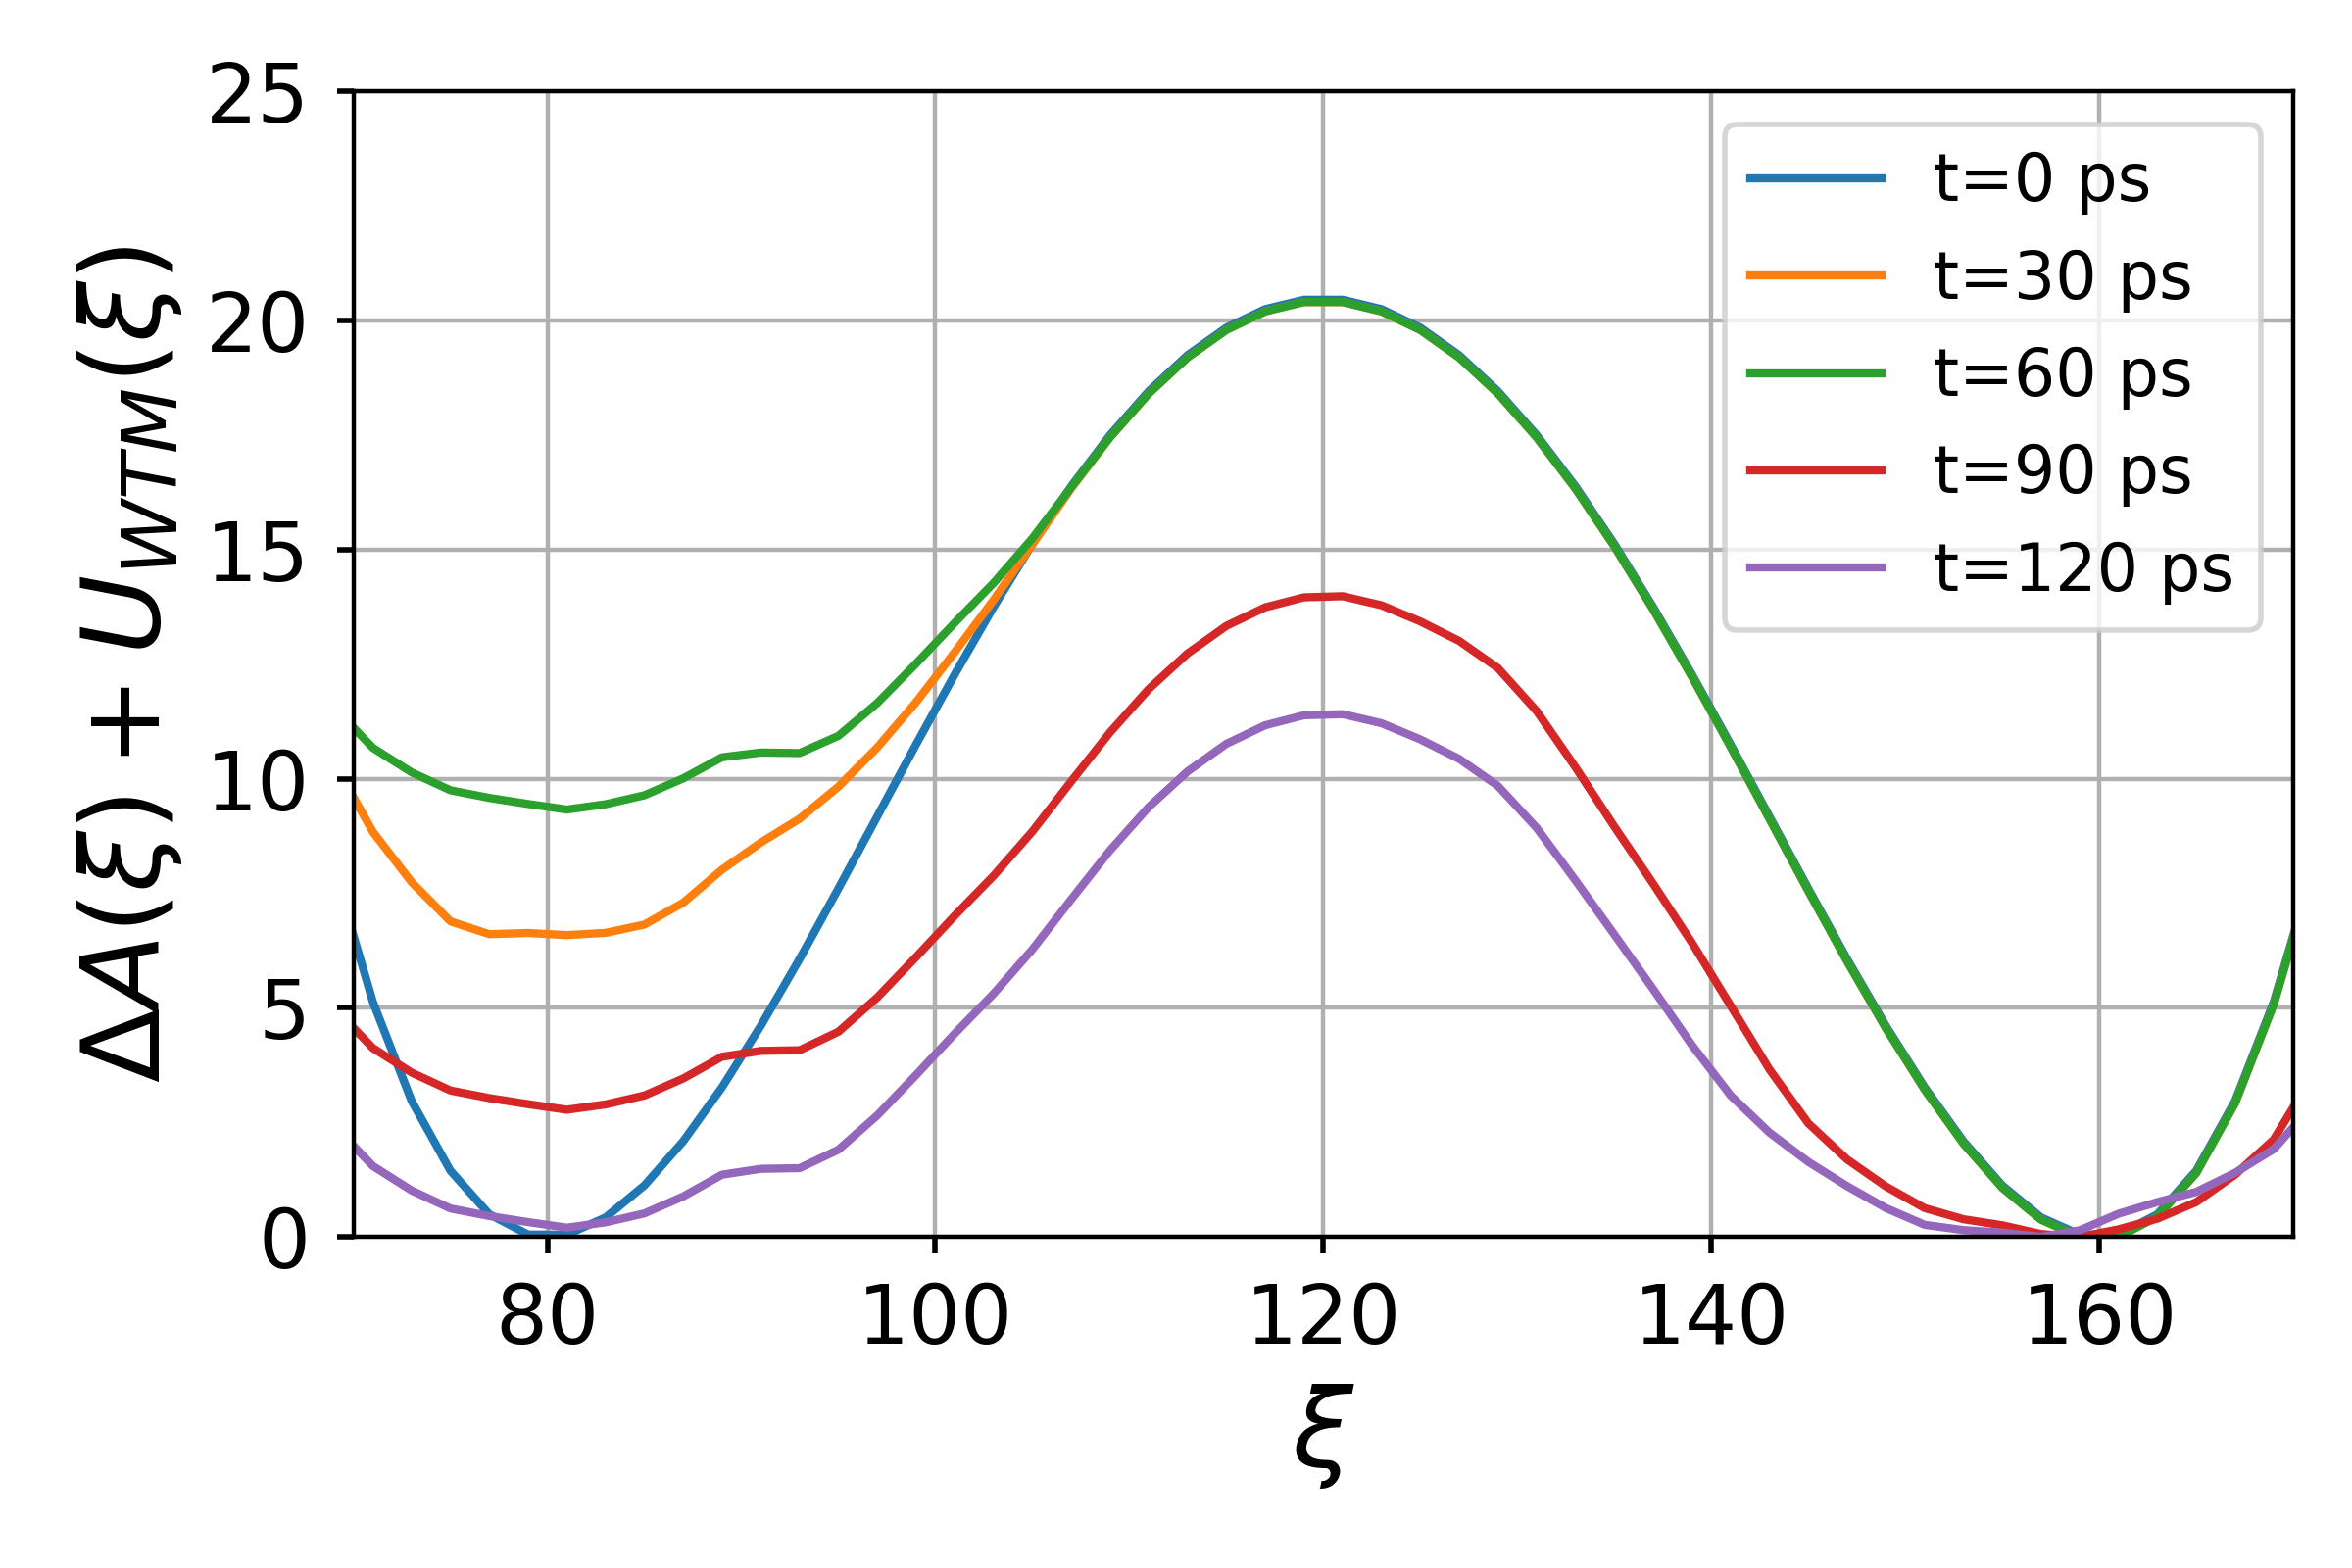
\includegraphics[width=0.49\textwidth]{bilder/WTM_eff_pot} }}
    \caption{Numerical example of the metaD and WTM algorithm for a particle in a 2D double well potential. The reaction coordinate $\xi$ is the x-direction. Over time the bias potentials $U_{MtD}$ and $U_{WTM}$ build up and reduce the free energy barrier. $U_{MtD}$ will ultimately completely remove the free energy barrier, whereas $U_{WTM}$ converges to a certain limit, which can be controlled with parameter $\Delta T$. Details are given in the Appendix.}
\label{fig:metaD}%
\end{figure}

\subsection{Adaptive Biasing Force Method (ABF)}
\label{sec:ABF}

The intuition behind ABF is, that adding a force $\frac{\partial A(\textbf{x})}{\partial \xi}\nabla\xi(\textbf{x})$ that exactly compensates the average of the original force $-\nabla U(\textbf{x})$ along a given coordinate would result in uniform sampling along this coordinate.\autocite{comer2015adaptive}
Historically, this idea emerged from thermodynamic integration (TI), were the free energy derivative  is computed as the ensemble average of the instantaneous force, $F$, acting along the collective variable:
\begin{equation}
\frac{dA}{d\xi} = -\braket{F}_{\xi}
\end{equation}
and the free energy is calculated as the integral over this force.\autocite{kirkwood1935statistical,zwanzig1954high}
In practice, as one has no prior knowledge of the free energy derivative, ABF uses an on-the-fly estimate of the mean force acting along the reaction coordinate. For this purpose the transition coordinate $\xi$, connecting two end points, is divided in $M$ equally spaced bins. The approximation of the bias force $\overline{F}(N,k)$ in bin $k$ is than the average of collected force samples:\autocite{comer2015adaptive}
\begin{equation}
  \overline{F}(N,k) = \frac{1}{N^{k}} \sum_{\mu=1}^{N^{k}} F_{\mu}^{k}
  \label{eq:mean force}
\end{equation}
At the beginning of the simulation $\overline{F}$ is scaled up by a linear ramp function $R(N^k)$ to prevent large fluctuations of the force estimate from driving the system away from equilibrium.
\begin{equation}
  R(N^k)=\left\{\begin{array}{ll} N_{full}, & N^{k} < N_{full} \\
                                           1, & N^{k} \geq  N_{full} \end{array}\right. \label{eq:ramp}
\end{equation}
The number of samples when the full biasing force is applied, $N_{full}$, and the bin size are the only free parameters.
It can be proven mathematically, that equation \ref{eq:mean force} converges (under some constraints exponentially) to $-dA/d\xi$ for a sufficiently large number of force samples.\autocite{alrachid2015long}
Figure~\ref{fig:ABF} shows a numerical example for the flattening of the reaction coordinate during an ABF simulation.

\begin{figure}[H]
    \centering
    \subfloat[ABF force $\overline{F}$]{{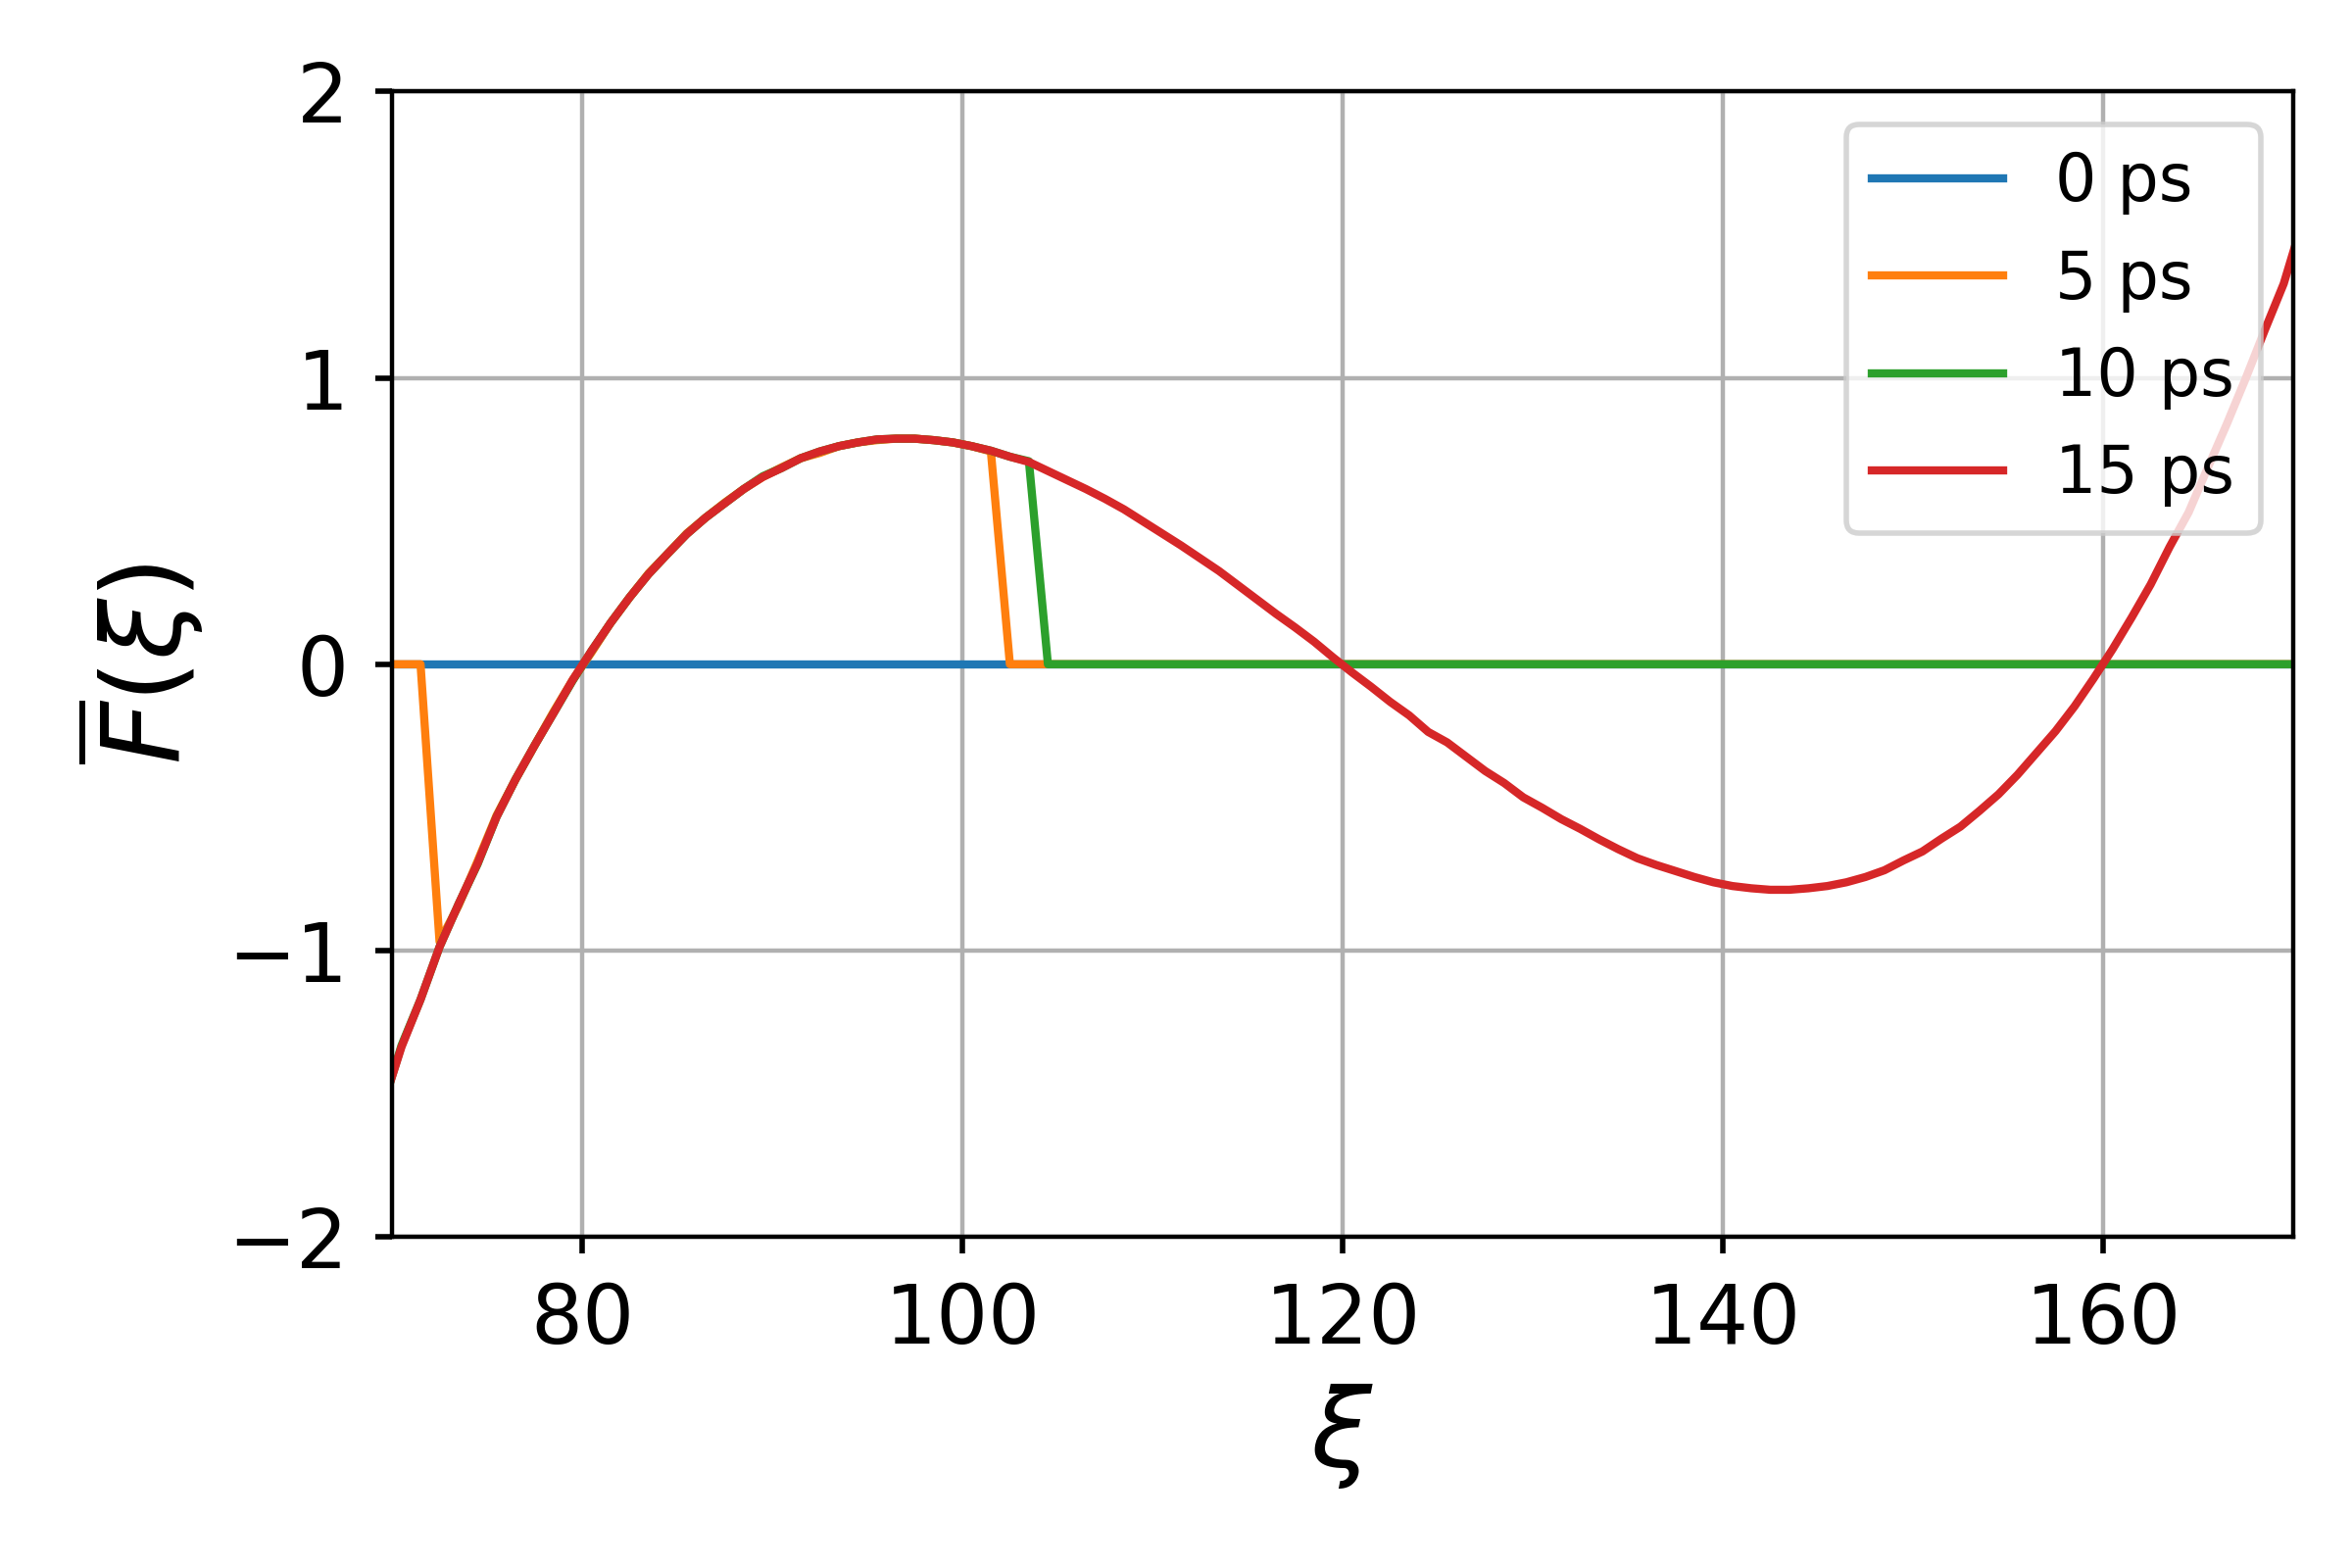
\includegraphics[width=0.49\textwidth]{bilder/ABF_force} }}
    \subfloat[effective potential ($A(\xi)-\int\overline{F}(\xi)d\xi$) during ABF simulation ]{{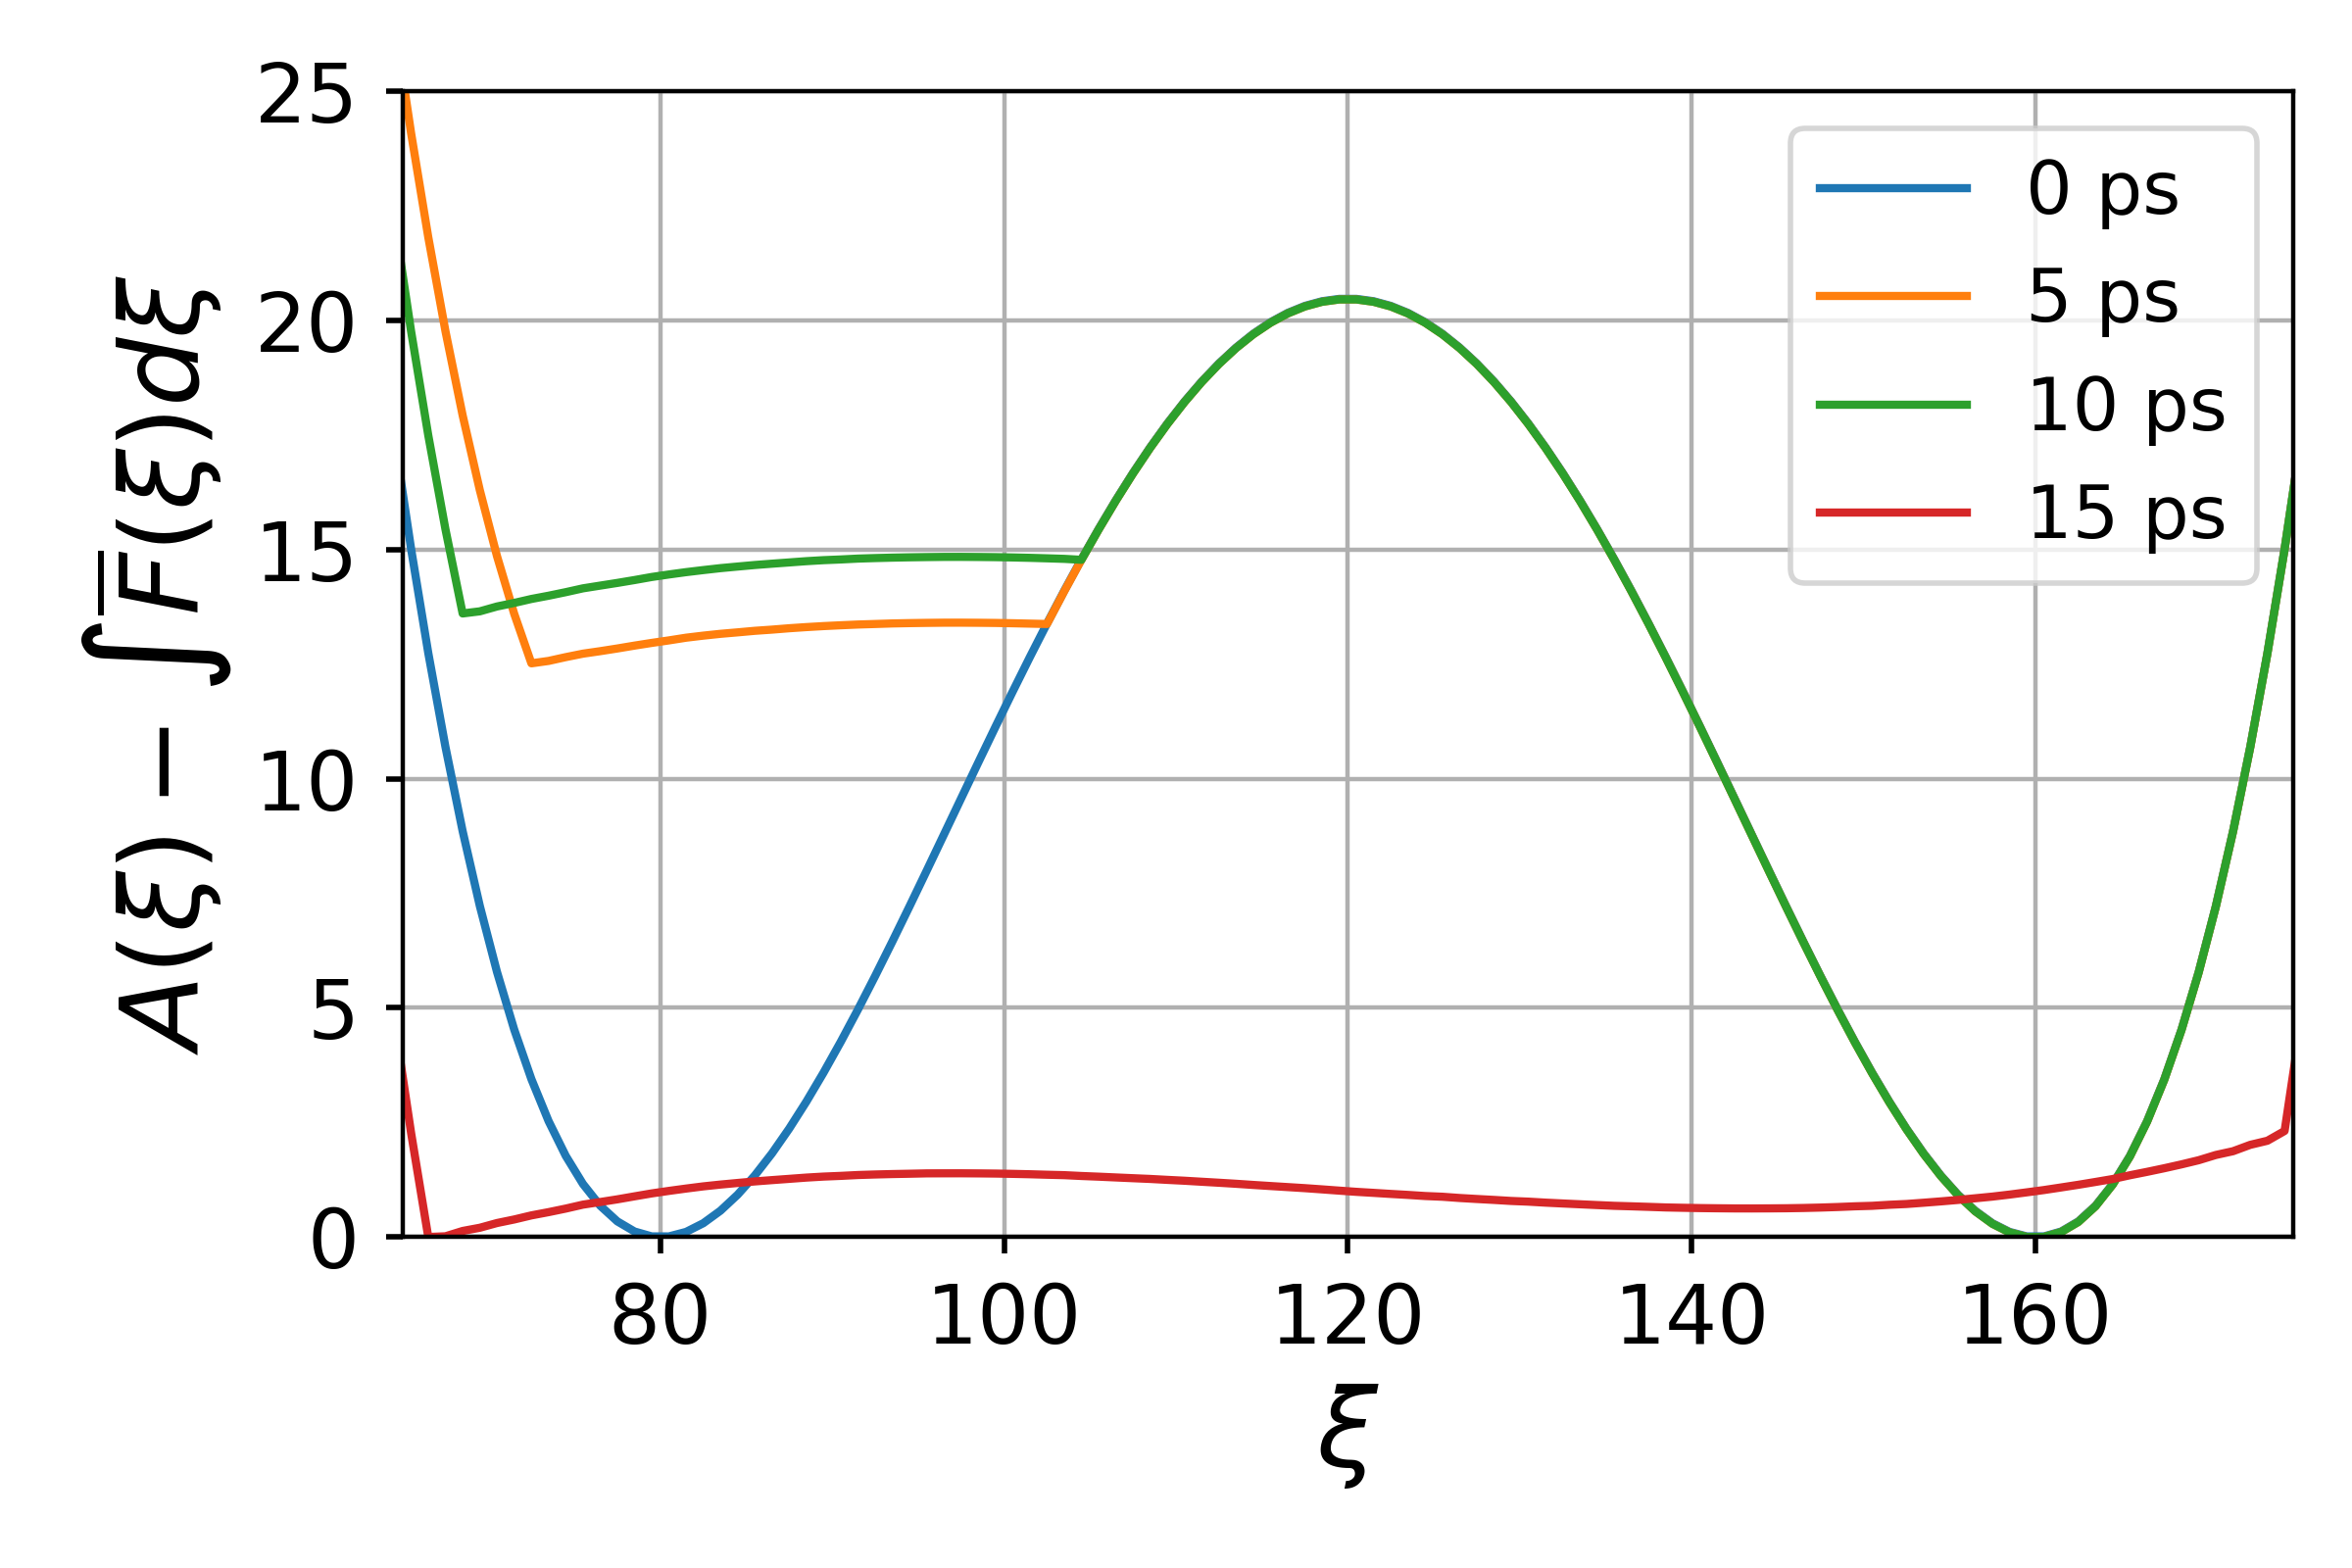
\includegraphics[width=0.49\textwidth]{bilder/ABF_freeE} }}
    \caption{Numerical example of ABF algorithm for 2D double well potential. The reaction coordinate $\xi$ is the x-direction. $\overline{F}(\xi)$ completely compensates the free energy barrier after 15~ps. From there on the system evolution resembles Brownian motion along the flattened reaction coordinate, which will ultimately lead to uniform sampling. Details are given in the Appendix.}
\label{fig:ABF}%
\end{figure}

For 1D reaction coordinates the unbiased free energy difference $A$ can be trivially obtained from $\overline{F}$ with any numerical integration scheme (e.g. Simpson's rule).
However, this is not true for multidimensional reaction coordinates, because $\overline{F}$ is no conservative force due to statistical errors. With simple integration the result would therefore depend on the integration path, which is physically incorrect. This problem can be avoided by using the \textit{finite element method} (FEM).\autocite{darve2008adaptive} For this purpose tent functions $B_l$ are used to approximate $A(\xi)$
\begin{equation}
  A(\xi) = \sum_l \alpha_l B_l(\xi)
\end{equation}
where the coefficients $\alpha_l$ are obtained by minimizing
\begin{equation}
  RMSD(\vec{\alpha})=\sqrt{\frac{1}{M}\sum_k^M\biggl(\bigl(\sum_l \alpha_l \nabla B_l(\xi_k)\bigr) - \braket{F(\xi_k)} \biggr)^2}
\end{equation}
with some numerical minimization routine (e.g. BFGS algorithm\autocite{nocedal2006numerical}) for force estimates of each dimension. An 1D example of the approximation of an arbitrary function by tent functions is given in \ref{fig:FEM}a. To increase the smoothness of the reconstructed free energy surface in practice four control points per bin and dimension are chosen between data points, as shown in figure \ref{fig:FEM}b.
\begin{figure}[H]
    \centering
    \subfloat[Example of 1D tent functions $B_l(\xi)$ (colored) approximating an arbitrary free energy surface $f(\xi)$ (blue)]{{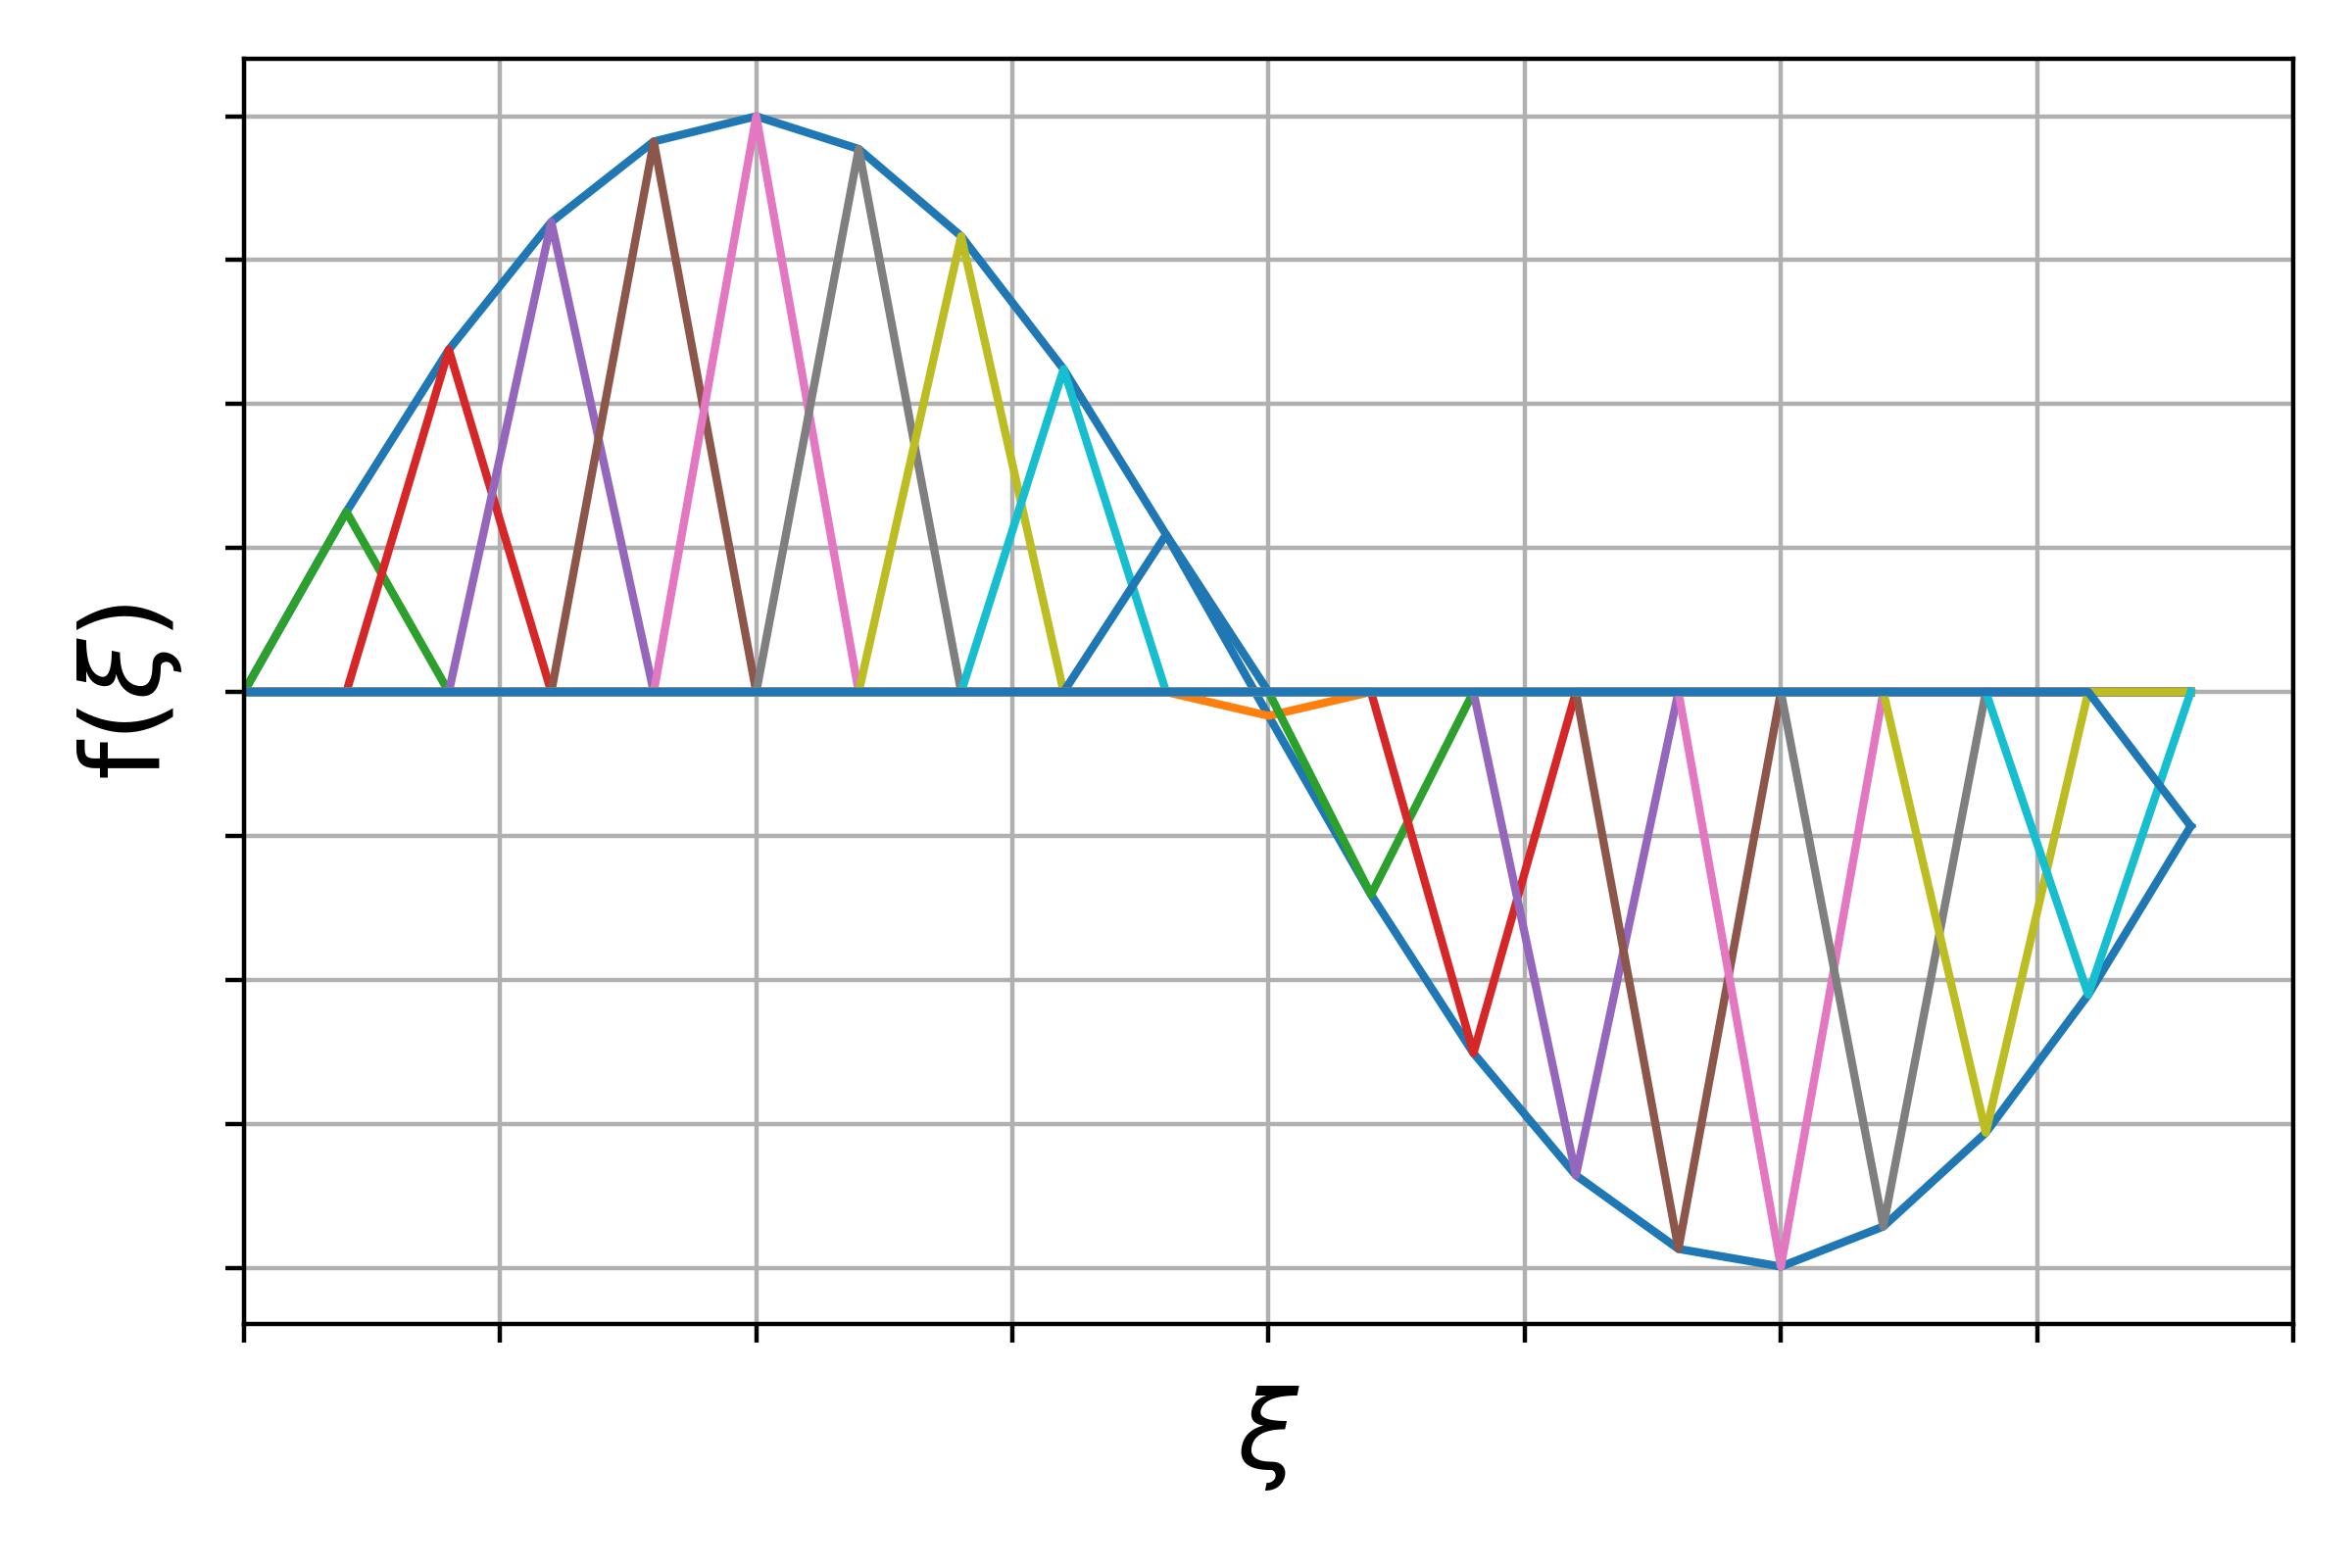
\includegraphics[width=0.44\textwidth]{bilder/FEM_1D} }}
    \subfloat[Illustration of numerical grid used for FEM integration of ABF-forces in 2D. Blue are original data points and orange control points obtained by linear interpolation. One 2D tent function is centered on each blue point.]{{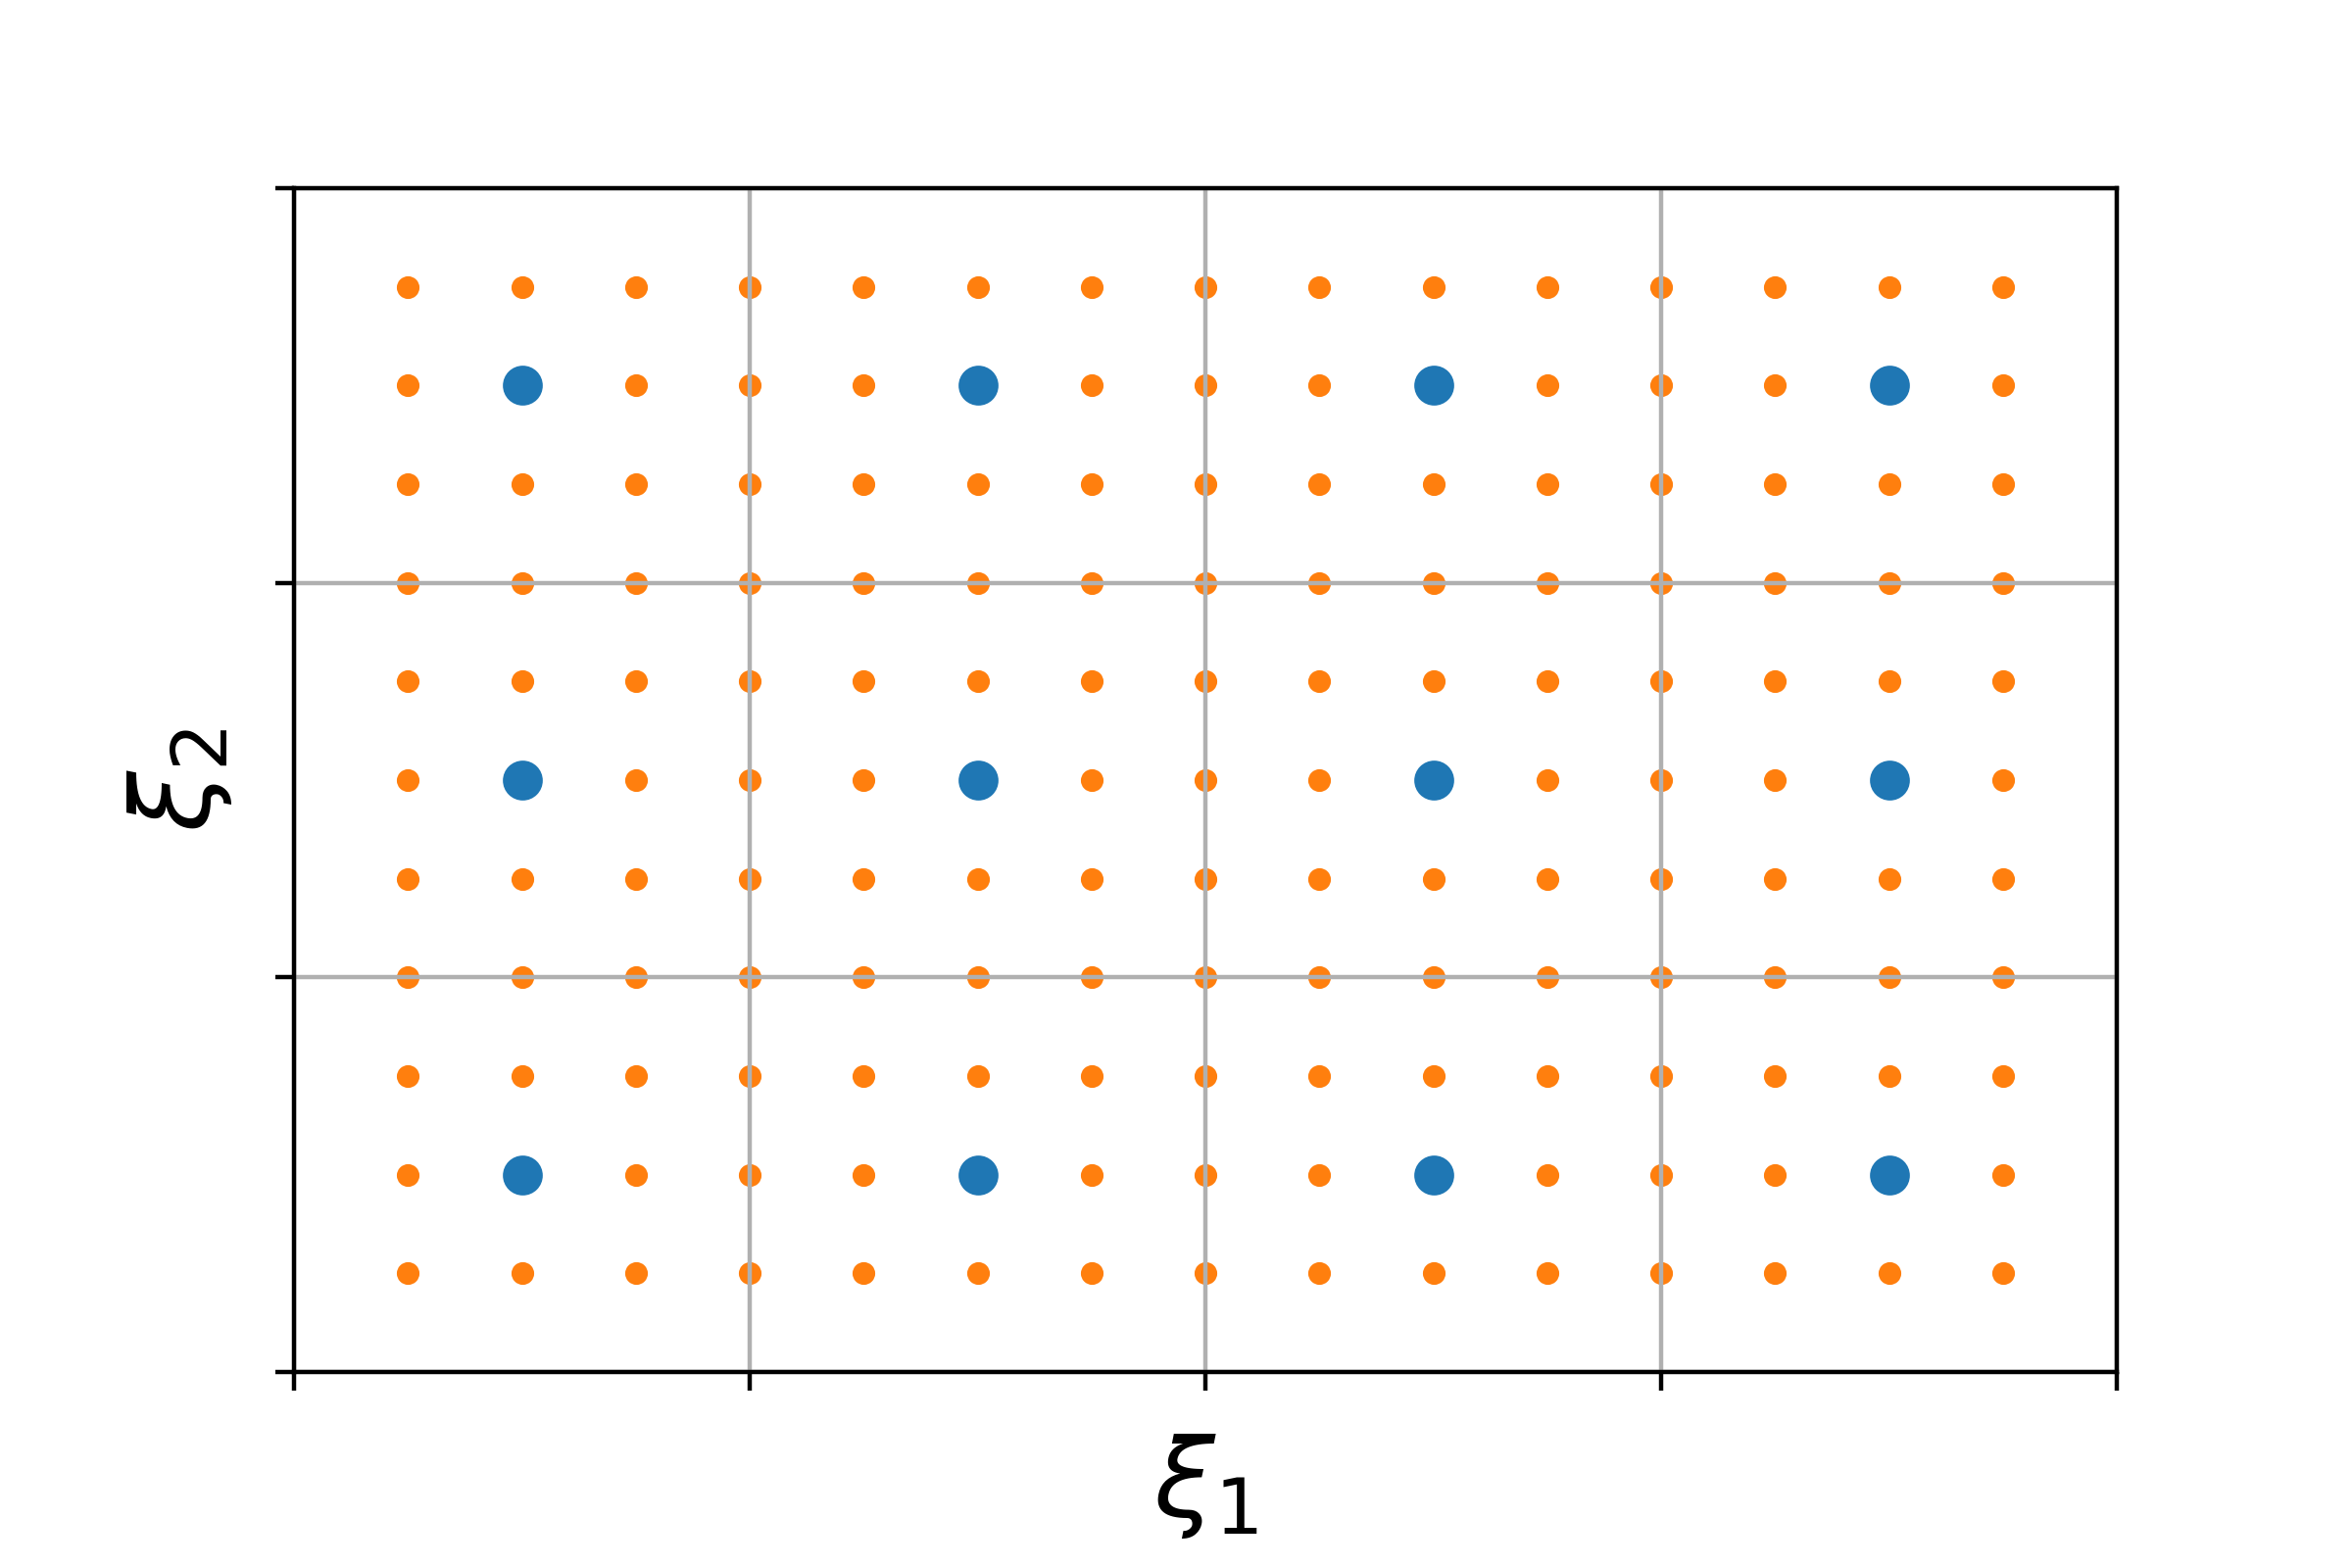
\includegraphics[width=0.49\textwidth]{bilder/grid} }}
    \caption{Illustration of the FEM integration}
\label{fig:FEM}%
\end{figure}
The last missing ingredient for the ABF method is an explicit expression for the instantaneous force samples $F_{\xi}$. Carter et al.\autocite{carter1989constrained} gave a first general expression:
\begin{equation}
  F(\xi,\textbf{q}) = -\frac{\partial U(\xi,\textbf{q})}{\partial \xi} + \beta^{-1} \frac{\partial \ln|J(\xi,\textbf{q})|}{\partial\xi} \label{eq:instforce old}
\end{equation}
which depends implicitly on a vector field $\partial x_i / \partial \xi$, hereafter referred to as "inverse gradient" and on an Jacobian correction term purely geometric in origin. The inverse gradient can be thought of as direction along which an infinitesimal change in $\xi$ is propagated in Cartesian coordinates, the complementary coordinates $\textbf{q}$ being kept constant. A major drawback of this formalism is the requirement of an full coordinate transform from Cartesian coordinates ($\textbf{x}$) to generalized coordinates ($\xi$, $\textbf{q}$).

This requirement could be lifted by den Otter\autocite{den2000thermodynamic}, who put forward the idea that the change in $\xi$ can be propagated along an arbitrary vector field $\textbf{v}_i$ ($\mathbb{R}^{3N} \to \mathbb{R}^{3N}$), provided it satisfies some orthonormality conditions.
Extended to multidimensional reaction coordinates \textbf{$\xi$} = ($\xi_i$) and in presence of a set of constraints $\sigma_{k}(\textbf{x})=0$ these read:\autocite{ciccotti2005blue}
\begin{equation}
  \textbf{v}_i \cdot \nabla \xi_j = \delta_{ij} \label{eq:cond1}
\end{equation}
\begin{equation}
  \textbf{v}_i \cdot \nabla \sigma_k = 0 \label{eq:cond2}
\end{equation}
If all reaction coordinates $\xi_i$ are orthogonal to one another and to all constraints, $\textbf{v}_i = \nabla \xi_j/|\nabla \xi_j|^2$ is always a valid option, but not necessarily the best.
Otherwise conditions \ref{eq:cond1} and \ref{eq:cond2} can be fulfilled by orthogonalization:\autocite{ciccotti2005blue}
\begin{equation}
  \textbf{v}_i (\textbf{x}) = \frac{Q^i \nabla \xi_i (\textbf{x})}{|Q^i \nabla \xi_i (\textbf{x})|} \label{eq:ortho v}
\end{equation}
with projector $Q^i$ given by the orthonormal basis $\{\hat{n}|_{j}^{i}(\textbf{x})\}_{j\neq i}$ in the subspace spanned by $\{\nabla \xi_j (\textbf{x})|\}_{j\neq i} \cup \{\nabla\sigma_j (\textbf{x})|\}_{j=1,...,M}$:
\begin{equation}
  Q^i = \textbf{1} - \sum_{j \neq i} \hat{n}_{j}^{i}(\textbf{x}) \otimes \hat{n}_{j}^{i}(\textbf{x})
\end{equation}
Replacing the inverse gradient by vectorfield $\textbf{v}_i$, expression \ref{eq:instforce old} finally reduces to:
\begin{equation}
  F(\xi_i,\textbf{x}) = -\nabla U(\textbf{x}) \cdot \textbf{v}_i(\textbf{x}) + \beta^{-1} \nabla \cdot \textbf{v}_i(\textbf{x}) \label{eq:inst ABF force}
\end{equation}
but still involves the calculation of second derivatives in the form of the divergence of vector fields $\textbf{v}_i$.\autocite{comer2015adaptive} Analytic expressions for distances, projected distances, bend angles and torsion angles, used in the present work, are given in the appendix. However, for complicated CV's like torsion angles orthogonalization via equation \ref{eq:ortho v} becomes exceedingly tedious and impractical, significantly limiting the applicability of ABF for multidimensional reaction coordinates.

\newpage
\subsection{extended Lagrangian based methods (eABF, meta-eABF, WTM-eABF)}
\label{sec:eABF}
To circumvent the technical requirements of ABF Lesage et al.\autocite{lesage2017smoothed} proposed an more flexible approach termed extended ABF (eABF), where additional coordinates $\lambda_i$ with mass $m_{i}$, which are coupled to reaction coordinates $\xi_i$ with harmonic potentials, are introduced. The extended system ($\textbf{x}$, $\lambda$) evolves according to Langevin dynamics in the potential
\begin{equation}
  U_{ext}(\textbf{x},\lambda) = U(\textbf{x}) + \sum_i^n \frac{(\xi_{i}(\textbf{x})-\lambda_i)^2}{2\sigma_i^2}.
\end{equation}
where the mass of the fictitious particle $m_i$ and the variance between extended coordinate and physical coordinate $\sigma_i^2=(\beta k_i)^{-1}$ are free parameters.
The key intuition behind eABF is, that in the tight coupling (low $\sigma$, high $k$) limit efficient sampling of $\lambda$ will result in efficient sampling of $\xi$.
Therefore, to obtain uniform sampling along $\xi$ it is sufficient to bias the dynamics of $\lambda$. The inverse gradient is chosen as zero for all physical coordinates $\textbf{x}$ and 1 for $\lambda$.
This way constraints \ref{eq:cond1} and \ref{eq:cond2} are always satisfied, which is especially useful for calculations involving a set of non-orthogonal reaction coordinates.
In practice the Langevin integrator for the extended system is implemented separately from the physical MD engine and can be coupled to any collective variable of interest without additional effort.

Sampling the extended system in thermal equilibrium gives the following Boltzmann distribution in $\lambda$:
\begin{equation}
  p_\lambda(\lambda) \propto \int \e^{-\beta U_{ext}(\textbf{x},\lambda)} d\textbf{x} \\
\end{equation}
The bias on $\lambda$ is the running average over the spring force in $\lambda$-bin k:
\begin{equation}
  \overline{F}(\lambda_{i}, k) = \frac{\partial A^{k}(\lambda_{i})}{\partial \lambda_i} = \frac{1}{N^{k}\sigma_i^2} \sum_{\mu=1}^{N^{k}} (\lambda_{i,\mu}^{k}-\xi_{i,\mu}^{k})
  \label{eq:eABF bias}
\end{equation}
Note that the instantaneous force estimate in each step no longer depends on the all atomic coordinates $\textbf{x}$ like in normal ABF (cf. equation \ref{eq:inst ABF force}), but only on ($\lambda_i - \xi_i$).
This has the advantageous side effect, that the noise in $\overline{F}$ can be reduced significantly and faster convergence of $\overline{F}$ can be expected, if $\sigma^2$ is well chosen.\autocite{lesage2017smoothed} Specifically, the mean square fluctuation of the spring force is proportional to $(\beta\sigma)^{-1}$, which shows that the variance of $\overline{F}$ is smaller for higher values of $\sigma$.
For small values of $N^{k}$ the linear ramp function $R(N,k)$ given by equation \ref{eq:ramp} is used nonetheless. Overall, with the time dependent bias converging towards $A(\lambda_{i})$, the biased Boltzmann distribution is given by:
\begin{equation}
  \tilde{p}_\lambda(\lambda_i) \propto \int \e^{-\beta U_{ext}(\textbf{x},\lambda_i) + A(\lambda_i)} d\textbf{x}
\end{equation}
We now need to find a robust estimator to recover the unbiased free energy of the physical system $A(\xi_i)$ from biased dynamics in the extended system.
The naive approach is to approximate $A(\xi_i)$ with $A(\lambda_i)$, which can be obtained by simply integrating the bias force $\overline{F}(\lambda_{i})$ like in normal ABF.
However, this will only produce unbiased results in the tight coupling limit for $\sigma \rightarrow 0$, where standard ABF is recovered.

An asymptotically unbiased estimator of the free energy can be derived by correcting the free energy gradient obtained from the eABF-biased distribution $\tilde{p}(\xi)$ with the average biasing force on $\xi$
\begin{equation}
  \frac{\partial A(\xi_i)}{\partial \xi_i} = -\beta^{-1}\frac{\partial \ln \tilde{p}(\xi_i)}{\partial \xi_i} + k(\braket{\lambda_i}_{\xi_i}-\xi_{i}) \label{eq:CZAR}
\end{equation}
which is called \textit{Corrected z-averaged restraint} (CZAR) and can be calculated on-the-fly during the simulation at little extra cost by introducing two additional accumulators for $\tilde{p}(z)$ and $k(\braket{\lambda_i}_{z}-z_{i})$ which are only joined at output times.\autocite{lesage2017smoothed} Figure \ref{fig:eABF traj} gives a numerical example for the application of eABF and figure \ref{fig:eABF flowchart} shows a schematic overview of the full eABF/CZAR algorithm.

\begin{figure}[H]
    \centering
    \subfloat[Snapshot of trajectories of $\xi$ and $\lambda$, \\
    Inset: Gaussian kernel for distance of $\xi$ and $\lambda$ with varinace $\sigma$]{{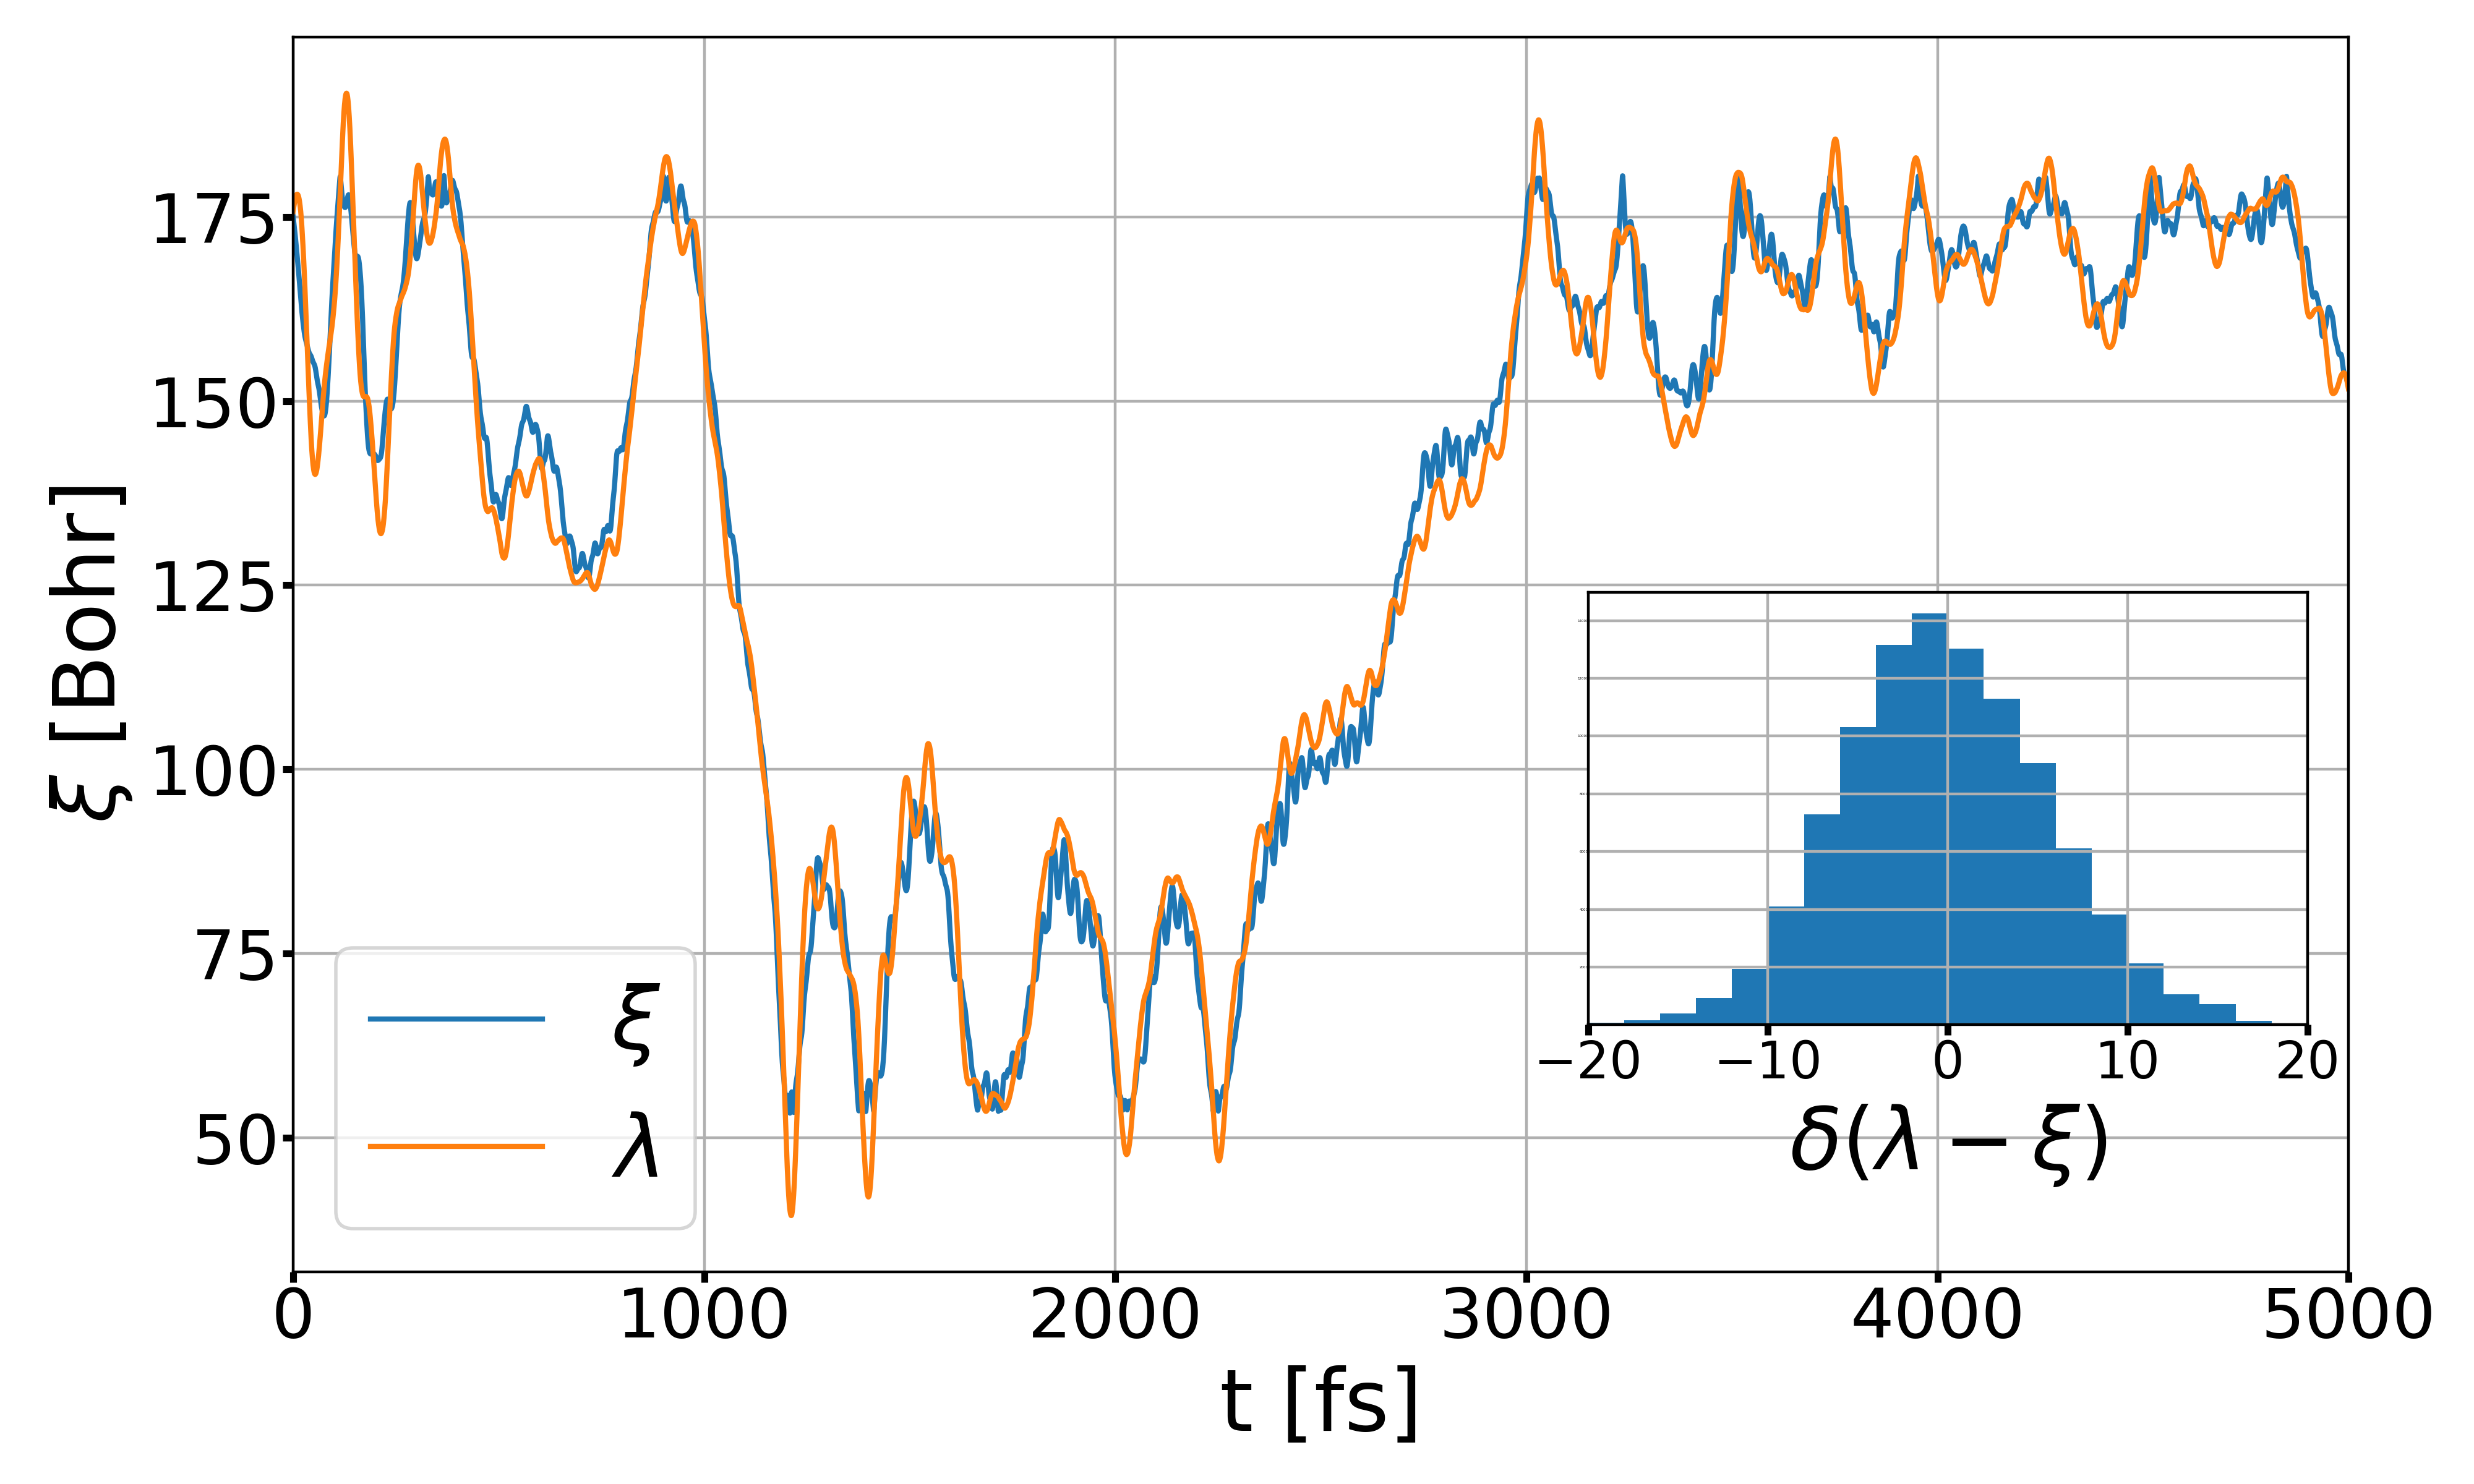
\includegraphics[width=0.49\textwidth]{bilder/eABF_traj} }}
    \subfloat[Free energy obtained by ABF, eABF with naive estimator and eABF with CZAR estimator]{{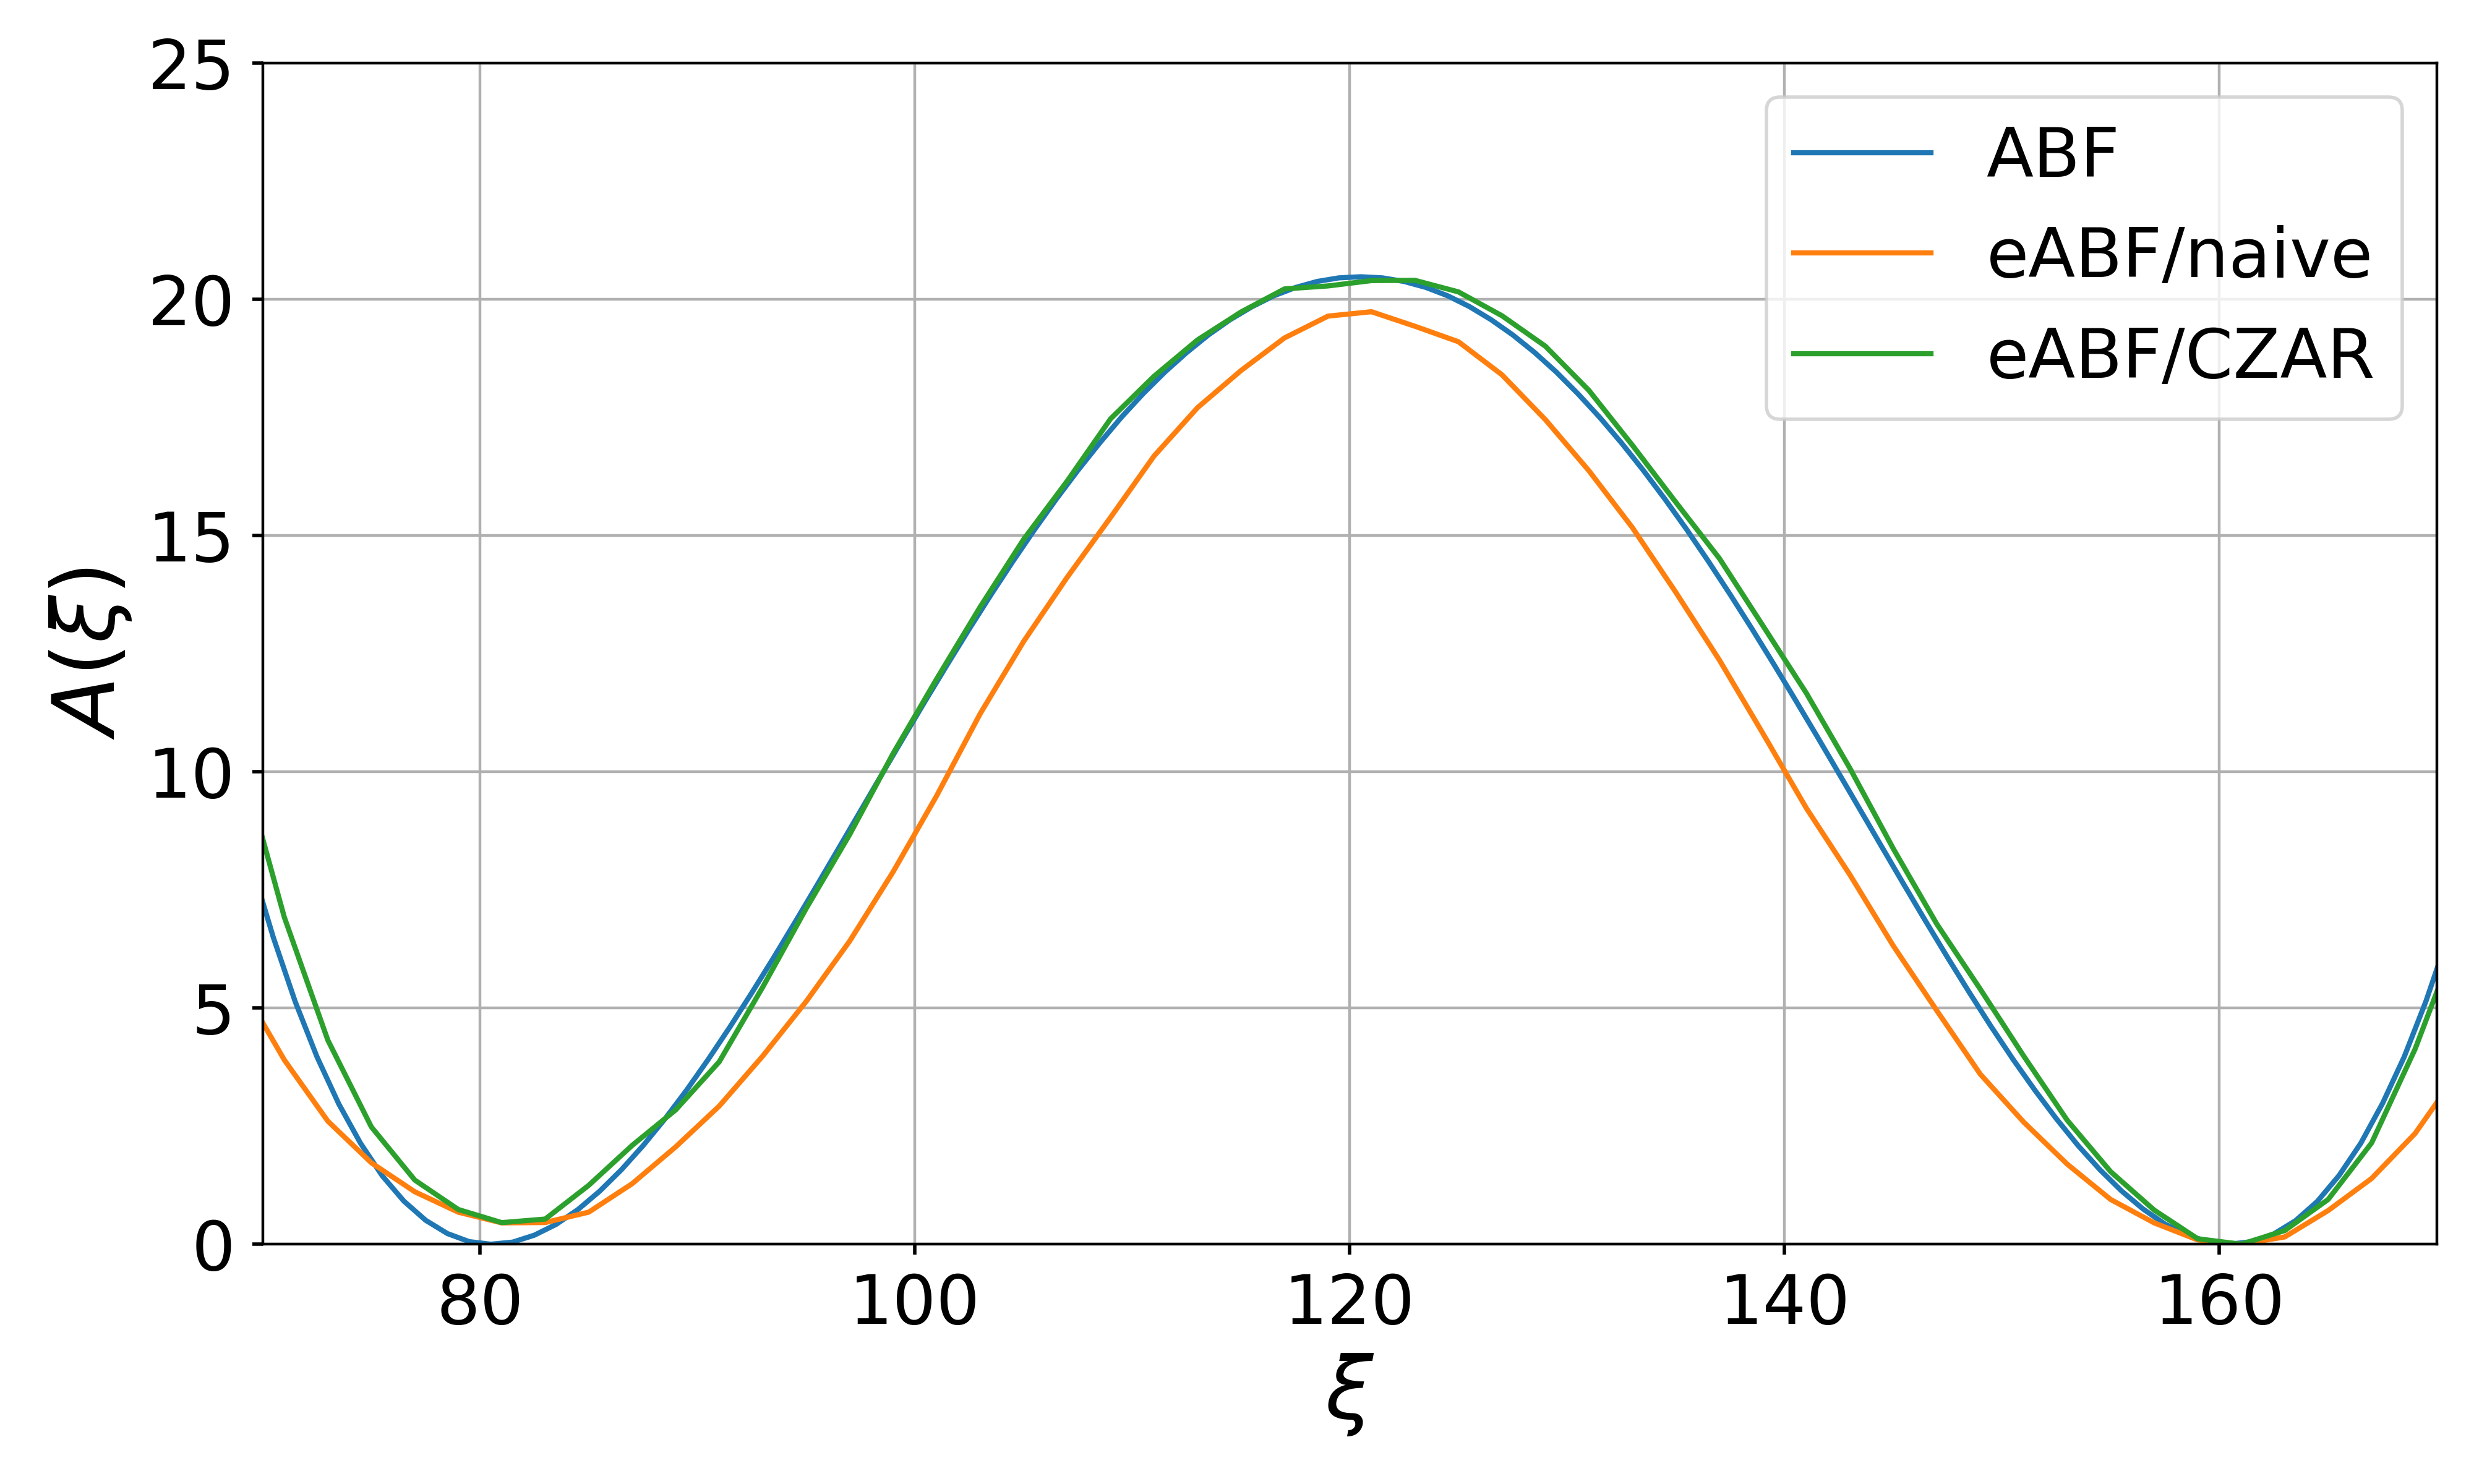
\includegraphics[width=0.49\textwidth]{bilder/eABF_freeE} }}
    \caption{Numerical examples for eABF algorithm with $m_\lambda=20$~a.u. and $\sigma=7$~Bohr. The reaction coordinate $\xi$ is the x-direction. }
\label{fig:eABF traj}%
\end{figure}

\begin{figure}[H]
   \caption{
     Flowchart of the eABF algorithm. $k_{\lambda,\xi}$ denote $\lambda$ or $\xi$ conditioned bin indices in bins with size $\Delta\xi$. $\tilde{\rho}_\lambda$ and $\tilde{\rho}_\xi$ are $\lambda$- or $\xi$- conditioned histograms and $R$ is the ABF ramp function. $F_B$ is the sum bias force samples. Outputs are written in fixed intervals.
   }

        \centering
        \begin{tikzpicture}[minimum size=5mm,node distance=4cm and 7cm,>=stealth,bend angle=45,auto]
        \node [block] (xi) {$\xi \leftarrow f(\textbf{x})$};
        \node [block, below of=xi] (langevin) {Langevin dynamics of extended system};
        \node [block, below of=langevin,yshift=-0.5cm] (F_ext) {add harmonic force of extended system to QM/MM forces};

        \node [decision, below of=F_ext, yshift=-1cm] (decide_lambda) {$\xi_{min}\leq \lambda \leq \xi_{max}$};

        \node [block, below of=decide_lambda,xshift=-3cm] (la_bin) {$k_\lambda = \lfloor \frac{|\lambda - \xi_{min}|}{\Delta \xi} \rfloor$};
        \node [block, below of=la_bin] (la_hist) {$\tilde{\rho}_\lambda(k_\lambda) \pluseqq 1$};
        \node [block, below of=la_hist] (R) {$R(k_\lambda) = f(k_\lambda)$ (eq. \ref{eq:ramp})};
        \node [block, below of=R] (F_B1) {$F_B(k_\lambda)\pluseqq \frac{1}{\sigma^2}(\lambda-\xi)$};
        \node [block, below of=F_B1] (F_B2) {$F(\textbf{x},\lambda) \pluseqq \frac{R(k_\lambda)F_B(k_\lambda)}{\tilde{\rho}_\lambda(k_\lambda)}\nabla\lambda$};

        \node [block, right of=R,xshift=4cm] (conf1) {confine $\lambda$ to range of interest};

        \node [decision, below of=F_B2,xshift=3cm] (decide_xi) {$\xi_{min}\leq \xi \leq \xi_{max}$};

        \node [block, below of=decide_xi,xshift=-3cm] (xi_bin) {$k_\xi = \lfloor \frac{|\xi - \xi_{min}|}{\Delta \xi} \rfloor$};
        \node [block, below of=xi_bin] (xi_hist) {$\tilde{\rho}_\xi(k_\xi) \pluseqq 1$};
        \node [block, below of=xi_hist] (F_corr) {$F_{corr}(k_\xi) \pluseqq \frac{1}{\sigma^2}(\lambda-\xi)$};

        \node [block, right of=xi_hist,xshift=4cm] (conf2) {confine $\xi$ to range of interest};

        \node [block,below of=F_corr,xshift=3.5cm] (MD1) {Finish Langevin dynamics of extended system};

        \node [decision, left of=decide_xi,xshift=-5.5cm] (output) {write output?};
        \node [block, left of=F_B1,xshift=-6cm] (CZAR) {calculate CZAR according to eq. \ref{eq:CZAR}};
        \node [block, left of=la_bin,xshift=-6cm] (out) {write output};

        \node [block, above of=output,yshift=10cm] (MD2) {MD step of physical system. (compare Algorithm \ref{alg:ABM})};

        \path [line] (xi) -- (langevin);
        \path [line] (langevin) -- (F_ext);
        \path [line] (F_ext) -- (decide_lambda);

        \path [line] (decide_lambda) -- node [above,xshift=-0.3cm] {yes} (la_bin);
        \path [line] (la_bin) -- (la_hist);
        \path [line] (la_hist) -- (R);
        \path [line] (R) -- (F_B1);
        \path [line] (F_B1) -- (F_B2);

        \draw [->] (decide_lambda) -- node {no} (conf1);

        \path [line] (F_B2) -- (decide_xi);
        \path [line] (conf1) -- (decide_xi);

        \draw [->] (decide_xi) -- node [above,xshift=-0.3cm] {yes} (xi_bin);
        \path [line] (xi_bin) -- (xi_hist);
        \path [line] (xi_hist) -- (F_corr);

        \draw [->] (decide_xi) -- node {no} (conf2);

        \path [line] (F_corr) -- (MD1);
        \path [line] (conf2) -- (MD1);

        \path [line] (MD1) -| (output);
        \path [line] (output) -- node [below,yshift=-0.2cm] {yes} (CZAR);
        \path [line] (CZAR) -- (out);
        \path [line] (out) -- (MD2);

        \draw[->] (output) -- node {no} (MD2);
        \draw[->] (MD2) |- (xi);

        \end{tikzpicture}
        \label{fig:eABF flowchart}
\end{figure}

The CZAR estimator is able to recover the unbiased free energy derivative only from time trajectory $(z_i,\lambda_i)$ of the extended system, independent of the bias on $\lambda_i$, as long as the simulation is in thermal equilibrium. It is therefore possible to bias the extended variable with any arbitrary force, for example metadynamics (eMtd, eWTM).
One particular useful choice for $\overline{F}(\lambda_{i}, k)$ is to combine repulsive MtD or WTM potentials with the eABF bias, an idea the authors figuratively described with 'Shaving Barriers, and Flooding Valleys'.\autocite{fu2018zooming}
This way the inherent difficulty for ABF methods to get accurate force estimates in high free energy regions at the beginning of the simulation can be solved, by pushing the system towards this regions.
The full MtD-eABF and WTM-eABF bias terms read
\begin{equation}
  F_{B}^{MtD-eABF}(\lambda_i, t) = -\frac{\braket{\xi_i(\textbf{x})-\lambda_i}_{\lambda_i}}{\beta \sigma_i^2}+\frac{\partial}{\partial \lambda_i} U_{B}^{MtD}(\lambda_i,t)
\end{equation}
\begin{equation}
  F_{B}^{WTM-eABF}(\lambda_i, t) = -\frac{\braket{\xi_i(\textbf{x})-\lambda_i}_{\lambda_i}}{\beta \sigma_i^2}+\frac{\partial}{\partial \lambda_i} U_{B}^{WTM}(\lambda_i,t)
\end{equation}
with $U_{B}^{MtD}$ and $U_{B}^{WTM}$ given by equations \ref{eq:U_mtD} and \ref{eq:WTM}.
The relative contributions of the eABF and MtD/WTM term will fluctuate over the course of a simulation, but the sum of both will eventually converge. However, accurate evaluation of $F_B$ is not even required, because it only enhances sampling of the reaction coordinate and the true PMF is obtained independently from CZAR.

\subsection{Multiple-Walker (MW) strategy for adaptive biasing}
\label{sec:MW}
By using the previously described methods the required simulation time to sample the reaction coordinate of alchemical transitions can be reduced from multiple ns to few ps, reducing the required MD steps by roughly a factor of 1000.
However, instead of using only one single MD simulation, i.e. \textit{walker}, one can think of letting multiple walkers contribute to the same bias, to exploit the full potential of modern HPC clusters.
For this purpose all accumulators $f$ required for the respective method, such as histograms, bias forces or potentials, are synced between otherwise independent walkers in fixed time intervals. Global and local accumulators evolve according to the following update formula
\begin{equation}
   f_{l}(t_{sync}) \leftarrow f_{g} + \biggl(f_{l}(t_{sync})-f_{l}(t_{sync}-1) \biggr)
\end{equation}
\begin{equation}
   f_{g} \leftarrow f_{l}(t_{sync})
\end{equation}
with time of synchronization $t_{sync}$.
Global contributions $f_{g}$ are stored in a single buffer, which can only be accessed by one walker simultaneously to avoid inconsistencies.

\section{Calculating free energy barriers and reaction rate constants}
\label{sec:A_geom}
All methods described so far enable the efficient calculation of some CV-based FES, as defined in equation~\ref{eq:free energy}.
As already noted in section \ref{sec:freeE}, this formulation is not invariant under the transformation of CV, e.g. $A(\xi(\textbf{x}))\neq A(\zeta(\textbf{x}))$, which should not come as a surprise as $\exp(-\beta A(\xi))/Z$ and $\exp(-\beta A({\zeta})/Z$ gives the marginal distribution along $\xi$ or $\zeta$, respectively.
Critical points like local minima or saddle points of $A(\xi)$ have therefore no coordinate independent meaning and can not be used to obtain kinetic information, like free energy barriers $\Delta^\ddagger A_{A\rightarrow B}$ or reaction rate constants $k_{A\rightarrow B}$.\autocite{bal2020free}

However, there also exists a different free energy definition, invariant under CV transformation, which will hereafter be referred to as geometric free energy, $A^G(\xi)$.\autocite{hartmann2011two}
For this purpose the delta function of equation \ref{eq:rho} is replaced by a proper surface measure
\begin{equation}
  \rho^G (\xi) = \int \e^{-\beta U(\textbf{x})} d\xi(\textbf{x})
\end{equation}
and the geometric free energy is defined analogous to the normal free energy (equation \ref{eq:free energy})
\begin{equation}
  A^G(\xi) = -\beta^{-1}\ln \rho^G(\xi)
\end{equation}
Instead of the marginal distribution of the collective variable $\rho^G(\xi)$ is the probability density of the FES.
The statistical ensembles related to both free energy definitions can be augmented into one another by the Fixman correction term $U \mapsto U + \beta^{-1}\ln |\nabla \xi|$ which relates both free energies through the $\xi$-conditioned average of gradients using
\begin{equation}
  A^G(\xi) = A(\xi) - \beta^{-1}\ln\braket{\lambda |\nabla \xi|}_\xi
  \label{eq:f geom}
\end{equation}
where the length scale $\lambda$ is introduced to keep the exponential term dimensionless. Because all methods described in section \ref{sec:adaptive biasing} already involve calculation of the gradient this correction can be obtained with almost no additional effort.\autocite{bal2020free} For multidimensional CVs $\braket{\lambda|\nabla\xi|}_\xi$ is replaced by $\braket{\lambda^n \det d}_\xi$ with
\begin{equation}
  d^2_{ij} = \nabla \xi_i \cdot \nabla \xi_j
\end{equation}
Figure \ref{fig:F geom} gives an numerical example of the relation of $A^G$ and $A$ in an ABF simulation.
Using $A_G$ free energy barriers can be calculated that are independent of the choice of CV.
However, simply taking the difference $A_{TS}^G-A_{min}$ would still contain the partition function inside a volume element around the transition state.\autocite{bal2020free}
It therefore entails a dependence on the unit system of the simulation which finally has to be removed to obtain the free energy barrier according to
\begin{equation}
  \Delta^\ddagger A_{A\rightarrow B} = A_{TS}^G + \frac{n}{\beta}\ln \frac{\lambda}{h}\sqrt{\frac{2 \pi m}{\beta}}-A_{min}
\end{equation}
where $n$ is the number of dimensions of the CV and $h$ is the Planck constant. The mass factor $\sqrt{m}$ can be dropped by using mass scaled coordinates $\textbf{q}=\sqrt{m}\textbf{x}$. $\lambda$ than has the unit of $\textbf{q}$.
The reaction rate constant $k_{A\rightarrow B}$ can be obtained from the Eyring equation
\begin{equation}
  k_{A\rightarrow B} = \frac{\kappa}{h\beta}e^{-\beta \Delta^\ddagger A_{A\rightarrow B}}
\end{equation}
where $\kappa$ compensates the lowering of the reaction rate by recrossing of the transition state. However, in most chemical systems transport over the transition state can be assumed to be ballistic ($\kappa=1$).\autocite{bal2020free} Figure \ref{fig:F geom} gives an example of the connection of standard and geometric free energy.
\begin{figure}[H]
    \centering
    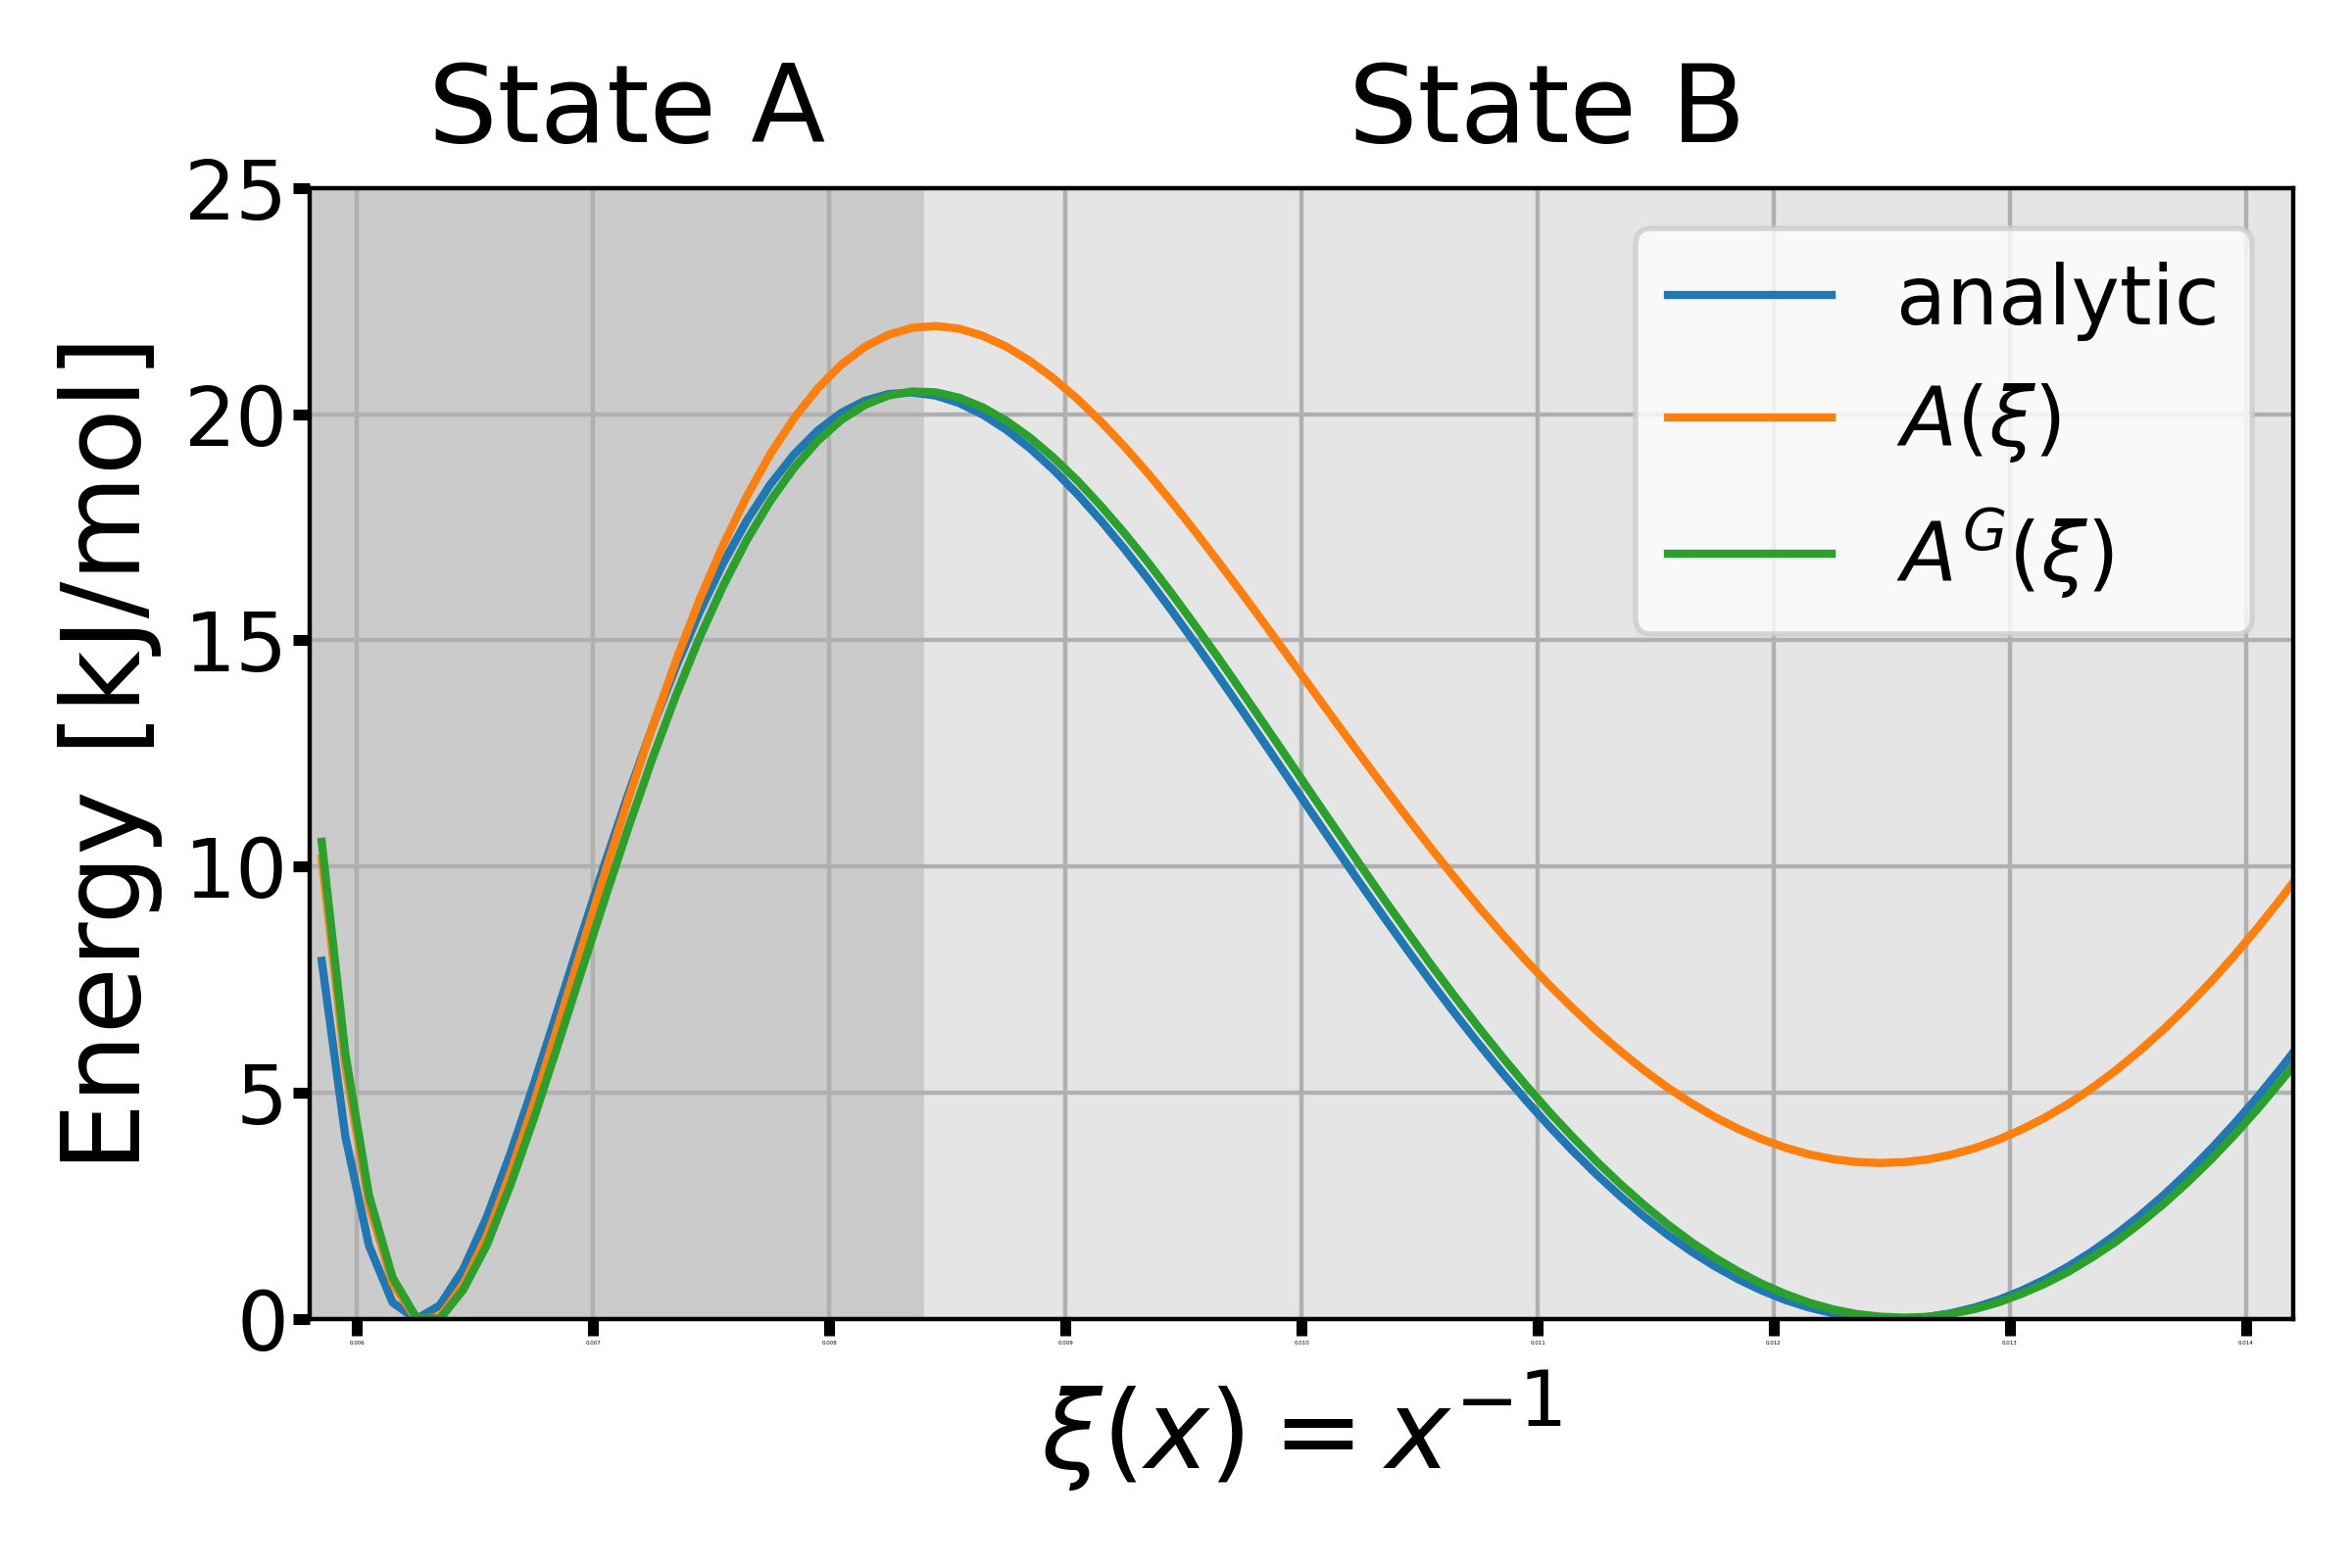
\includegraphics[width=0.6\textwidth]{bilder/geom_free_energy}
    \caption{
      Standard and geometric free energy of an 2D double well potential sampled along $\xi(x)=1/x$ using the ABF method.\\
      Both minima are equally probable, which is correctly described by the standard free energy difference $\Delta A_{A\rightarrow B}=-\beta^{-1}\ln \frac{\int_B \rho(\xi)d\xi}{\int_A \rho(\xi)d\xi}=0$.\\
      Correcting $A(\xi)$ according to equation \ref{eq:f geom} gives the geometric free energy $A^G$. In this example the geometric free energy surface is equal to the underlying potential energy surface $U(\xi)$. This is only true if the collective variable is adiabatically separable from the remaining degrees of freedom, in this case the y-direction.\autocite{hartmann2011two} Details are given in the Appendix.
    }
\label{fig:F geom}%
\end{figure}
